\باب{سمتیات اور خلا میں تحلیلی جیومیٹری}
اس حصہ میں سمتیات اور سہ بعدی محددی نظام متعارف کئے جائیں گے۔ جیسا ایک متغیر کے تفاعل پر غور کے لئے محددی مستوی موزوں ہے، اسی طرح دو (یا دو سے زیادہ) متغیرات کے تفاعل پر غور کے لئے محددی خلاء موزوں ہے۔ ہم محددی مستوی میں ایک تیسرا محور شامل کر کے محددی خلاء پیدا کرتے ہیں۔ یہ محور \عددی{xy} مستوی سے نیچے اور اس سے اوپر فاصلہ ناپتا ہے۔

\حصہ{مستوی میں سمتیات} 
بعض چیزیں جنہیں ہم ناپتے ہیں کا تعین ان کی مقدار سے ہوتا ہے۔مثال کے طور پر کمیت، لمبائی اور وقت قلم بند کرنے کے لئے  ہم صرف ایک عدد اور موزوں اکائی لکھتے ہیں۔ اس کے برعکس قوت، ہٹاو، یا سمتی رفتار جاننے کے لئے ہمیں مزید معلوم درکار ہو گی۔ قوت کو بیان کرنے کے لئے ہمیں اس کی مقدار کے ساتھ وہ رخ بھی جاننا ہو گا جس رخ یہ عمل کرتی ہے۔ کسی جسم کا ہٹاو بیان کرنے کے لئے ہمیں اس سمت کا ذکر کرنا ہو گا جس سمت یہ جسم حرکت کرتا ہے اور ساتھ اس فاصلہ کا ذکر کرنا ہو گا جتنا یہ طے کرتا ہے۔ ایک جسم کی سمتی رفتار بیان کرنے کے لئے ہم حرکت کی سمت اور جسم کی رفتار کی بات کرتے ہیں۔

وہ مقدار جس کی جسامت اور سمت دونوں ہوں کو عموماً تیر کے نشان سے ظاہر کیا جاتا ہے جہاں مقدار کے رخ کو  تیر کا رخ  مقدار  کی جسامت کو، موزوں اکائیوں میں، تیر کی لمبائی ظاہر کرتی ہے۔

تیر کے اس نشان کو \اصطلاح{سمتیہ} کہتے ہیں۔

\ابتدا{تعریف}
ایک مستوی میں کسی مخصوص رخ خط کو \اصطلاح{سمتیہ}\فرہنگ{سمتیہ}\حاشیہب{vector}\فرہنگ{vector} کہتے ہیں۔ دو سمتیات صرف اس صورت ایک دوسرے کے برابر یا یکساں ہوں گے جب ان کی مقداریں ایک جیسی ہوں اور ان کے رخ ایک جیسے ہوں۔
\انتہا{تعریف}
%===================

یوں اگر سمتیات کو ظاہر کرنے والے تیر  آپس میں متوازی ہوں، ان کی لمبائیاں ایک جیسی ہوں اور ان کا رخ بھی ایک جیسا ہو تب یہ ایک ہی  سمتیہ کو ظاہر کرتے ہیں۔اس  کتاب میں سمتیہ کو موٹی لکھائی میں رومن حروف تہجی، مثلاً   \عددی{\kvec{v}}،  سے ظاہر کیا جائے گا\حاشیہد{قلم و کاغذ استعمال کرتے ہوئے سمتیہ کو رومن حروف تہجی پر تیر کا نشان \عددی{\vec{v}} یا نصف تیر کا نشان
$\krightharpoonup{v}$
 ڈال کر ظاہر کیا جاتا ہے۔)}۔نقطہ \عددی{A} سے نقطہ \عددی{B} تک تیر کو ہم 
$\krightharpoonup{AB}$
 لکھیں گے۔

\ابتدا{مثال}\شناخت{مثال_سمتیہ_یکساں_چار}
چار تیروں کو شکل \حوالہ{شکل_مثال_سمتیہ_یکساں_چار} میں دکھایا گیا ہے جن کی لمبائیاں اور رخ ایک جیسی ہیں۔ یوں یہ چاروں ایک ہی سمتیہ کو ظاہر کرتے ہیں جس کو ہم درج ذیل لکھتے ہیں۔
\begin{align*}
\krightharpoonup{AB}=\krightharpoonup{CD}=\krightharpoonup{ON}=\krightharpoonup{EF}
\end{align*}
\انتہا{مثال}
%=====================
\begin{figure}
\centering
\begin{minipage}{0.45\textwidth}
\centering
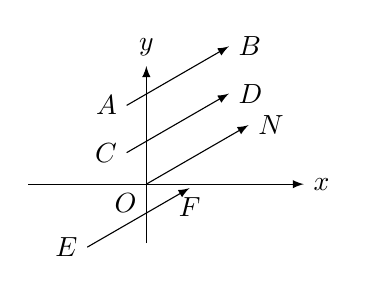
\begin{tikzpicture}
\pgfmathsetmacro{\k}{1.5}
\pgfmathsetmacro{\a}{30}
\draw[-latex](-1.5,0)--(2,0)node[right]{$x$};
\draw[-latex](0,-0.75)--(0,1.5)node[above]{$y$};
\draw[-latex](-0.25,1)node[left]{$A$}--++(\a:\k)node[right]{$B$};
\draw[-latex](-0.25,0.4)node[left]{$C$}--++(\a:\k)node[right]{$D$};
\draw[-latex](0,0)node[below left]{$O$}--++(\a:\k)node[right]{$N$};
\draw[-latex](-0.75,-0.8)node[left]{$E$}--++(\a:\k)node[below]{$F$};
\end{tikzpicture}
\caption{یکساں لمبائی اور یکساں رخ کے سمتیات ایک ہی سمتیہ کو ظاہر کرتے ہیں۔}
\label{شکل_مثال_سمتیہ_یکساں_چار}
\end{minipage}\hfill
\begin{minipage}{0.45\textwidth}
\centering
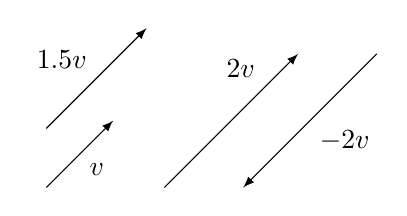
\begin{tikzpicture}
\pgfmathsetmacro{\k}{1.2}
\pgfmathsetmacro{\a}{45}
\draw[-latex](0,0)--++(\a:\k)node[pos=0.5,below right]{$\kvec{v}$};
\draw[-latex](0,0.75)--++(\a:1.5*\k)node[pos=0.5,above left]{$1.5\kvec{v}$};
\draw[-latex](1.5,0)--++(\a:2*\k)node[pos=0.75,above left]{$2\kvec{v}$};
\draw[latex-](2.5,0)--++(\a:2*\k)node[pos=0.5,below right]{$-2\kvec{v}$};
\end{tikzpicture}
\caption{سمتیہ کے غیر سمتی مضرب۔}
\label{شکل_سمتیہ_غیر_سمتی_مضرب}
\end{minipage}
\end{figure}
\جزوحصہء{غیر سمتیہ اور غیر سمتی مضرب}
ہم کسی سمتیہ کو مثبت حقیقی عدد سے ضرب دینے کے لئے اس کی لمبائی کو اس عدد سے ضرب دیتے ہیں (شکل \حوالہ{شکل_سمتیہ_غیر_سمتی_مضرب})۔ سمتیہ کو \عددی{2} سے ضرب دینے کے لئے ہم اس کی لمبائی دگنی کرتے ہیں۔ ایک سمتیہ کو \عددی{1.5} سے ضرب دینے کے لئے ہم اس کی لمبائی \عددی{\SI{50}{\percent}} بڑھاتے ہیں، وغیرہ، وغیرہ۔ ایک سمتیہ کو منفی  عدد سے ضرب دینے کے لئے ہم اس کا رخ الٹ کر کے اس کی لمبائی کو عدد کی مطلق قیمت سے ضرب دیتے ہیں۔

اگر \عددی{c} غیر صفر حقیقی عدد اور \عددی{\kvec{v}} ایک سمتیہ ہو تب مثبت \عددی{c} کی صورت میں \عددی{\kvec{v}} اور \عددی{c\kvec{v}} کے رخ ایک جیسے ہوں گے جبکہ منفی \عددی{c} کی صورت میں ان کے رخ ایک دوسرے کے مخالف ہوں گے۔ یہاں حقیقی اعداد تبدیلی پیمانہ کے طور پر کام کرتے ہیں اور یہ  \اصطلاح{غیر سمتی}\فرہنگ{غیر سمتی}\حاشیہب{scalar}\فرہنگ{scalar} کہلاتے ہیں جبکہ \عددی{c\kvec{v}} کے مضرب کو \عددی{\kvec{v}} کا \اصطلاح{غیر سمتی مضرب}\فرہنگ{غیر سمتی!مضرب}\حاشیہب{scalar multiple}\فرہنگ{scalar multiple} کہتے ہیں۔

صفر سے ضرب کو شامل کرنے کی خاطر ہم  اس روایت کو اپناتے ہیں جس کے  مطابق کسی بھی سمتیہ کو صفر سے ضرب دینے سے \اصطلاح{صفر سمتیہ} \عددی{\kvec{0}} حاصل ہو گا، جو ایک نقطہ پر مشتمل ہو گا جس کی لمبائی صفر ہو گی۔ دیگر سمتیہ کے برعکس صفر سمتیہ \عددی{\kvec{0}} کا کوئی رخ نہیں ہوتا ہے۔  

\جزوحصہء{جیومیٹریائی مجموعہ: قاعدہ متوازی الاضلاع}
دو غیر صفر سمتیات \عددی{\kvec{v}_1} اور \عددی{\kvec{v}_2} کا جیومیٹریائی مجموعہ لینے کی خاطر \عددی{\kvec{v}_1} کا نمائندہ، مثلاً \عددی{A} سے \عددی{B} تک، ترسیم کر کے \عددی{\kvec{v}_1} کے اختتامی نقطہ (سر) \عددی{B} پر \عددی{\kvec{v}_2}  کے نمائندہ کا ابتدائی نقطہ (دم)  رکھ کر ترسیم کریں۔ شکل \حوالہ{شکل_سمتیات_کا_مجموعہ} میں
$\kvec{v}_2=\krightharpoonup{BC}$
ہے۔ مجموعہ \عددی{\kvec{v}_1+\kvec{v}_2} اب \عددی{\kvec{v}_1} کے دم  \عددی{A} سے \عددی{\kvec{v}_2} کے سر  \عددی{C} تک سمتیہ ہو گا۔ یوں اگر
\begin{align*}
\kvec{v}_1=\overset{\rightharpoonup}{\rule{0pt}{.9ex}\smash{AB}},\quad \kvec{v}_2=\krightharpoonup{BC}
\end{align*}
ہوں تب
\begin{align*}
\kvec{v}_1+\kvec{v}_2=\krightharpoonup{AB}+\krightharpoonup{BC}=\krightharpoonup{AC}
\end{align*}
ہو گا۔چونکہ اس عمل میں \عددی{\kvec{v}_1+\kvec{v}_2} متوازی الاضلاع کا وتر ہوتا ہے لہٰذا اس عمل کو بعض اوقات \اصطلاح{قاعدہ متوازی الاضلاع}\فرہنگ{قاعدہ!متوازی الاضلاع}\حاشیہب{parallelogram law}\فرہنگ{law!parallelogram} کہتے ہیں (شکل \حوالہ{شکل_سمتیہ_قاعدہ_متوازی_الاضلاع})۔
\begin{figure}
\centering
\begin{minipage}{0.45\textwidth}
\centering
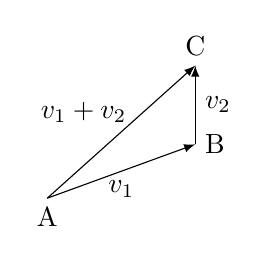
\begin{tikzpicture}
\draw[-latex](0,0)node[below]{A}--(20:2)node[pos=0.5,below]{$\kvec{v}_1$}node[right]{B};
\draw[-latex](20:2)--++(90:1)node[above]{C}node[pos=0.5,right]{$\kvec{v}_2$};
\draw[latex-](20:2)++(90:1)--(0,0)node[pos=0.4,left,yshift=0.5ex]{$\kvec{v}_1+\kvec{v}_2$};
\end{tikzpicture}
\caption{سمتیات \عددی{\kvec{v}_1} اور \عددی{\kvec{v}_2} کا مجموعہ۔}
\label{شکل_سمتیات_کا_مجموعہ}
\end{minipage}\hfill
\begin{minipage}{0.45\textwidth}
\centering
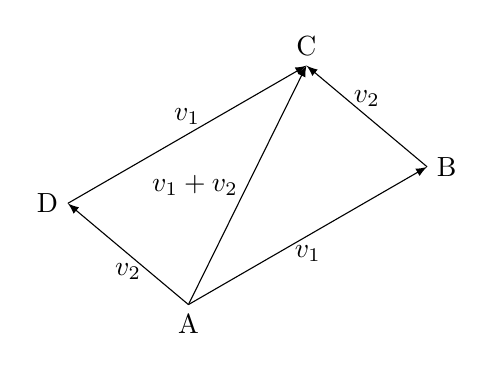
\begin{tikzpicture}
\pgfmathsetmacro{\da}{3.5}
\pgfmathsetmacro{\aa}{30}
\pgfmathsetmacro{\db}{2}
\pgfmathsetmacro{\ab}{140}
\draw[-latex](0,0)node[below]{A}--++(\aa:\da)node[right]{B}node[pos=0.5,below]{$\kvec{v}_1$}coordinate(kB);
\draw[-latex](kB)--++(\ab:\db)node[above]{C}node[pos=0.5,above]{$\kvec{v}_2$}coordinate(kC);
\draw[-latex](0,0)--++(\ab:\db)node[left]{D}node[pos=0.5,below]{$\kvec{v}_2$}coordinate(kD);
\draw[-latex](kD)--++(\aa:\da)node[pos=0.5,above]{$\kvec{v}_1$};
\draw[-latex](0,0)--(kC)node[pos=0.5,left]{$\kvec{v}_1+\kvec{v}_2$};
\end{tikzpicture}
\caption{قاعدہ متوازی الاضلاع۔ مخالف اضلاع یکساں لمبائی ہونے کی بنا \عددی{ABCD} متوازی الاضلاع ہو گا۔}
\label{شکل_سمتیہ_قاعدہ_متوازی_الاضلاع}
\end{minipage}
\end{figure}
\جزوحصہء{اجزاء}
دو سمتیات اس صورت متوازی ہوں گے جب یہ ایک دوسرے کے غیر صفر، غیر سمتی مضرب ہوں، یعنی جب ان کو ظاہر کرنے والے خطوط متوازی ہوں۔

جب بھی ایک سمتیہ \عددی{\kvec{v}} کو دو غیر متوازی سمتیات کا مجموعہ
\begin{align*}
\kvec{v}=\kvec{v}_1+\kvec{v}_2
\end{align*}
لکھنا ممکن ہو، سمتیات \عددی{\kvec{v}_1} اور \عددی{\kvec{v}_2} سمتیہ \عددی{\kvec{v}} کے اجزاء کہلائیں گے  اور ہم کہتے ہیں کہ  سمتیہ  \عددی{\kvec{v}} کو اس کے  اجزاء \عددی{\kvec{v}_1} اور \عددی{\kvec{v}_2} میں تحلیل کیا گیا ہے۔

سمتیات کے  مقبول ترین الجبرا میں ہر سمتیہ کو کارتیسی محور کے متوازی اجزاء کی صورت میں بیان کیا جاتا ہے اور یہ اجزاء از خود موزوں \اصطلاح{اساسی}\فرہنگ{اساسی}\حاشیہب{basic}\فرہنگ{basic} سمتیہ، جن کی لمبائی \عددی{1} ہوتی ہے، کے مضرب ہوتے ہیں۔ مثبت \عددی{x} محور کے رخ اساسی سمتیہ نقطہ \عددی{(0,0)} سے نقطہ \عددی{(1,0)} تک تیر سے ظاہر کیا جاتا ہے  اور اس اساسی سمتیہ کی علامت  \عددی{\ai} ہے۔ مثبت \عددی{y} محور کے رخ اساسی سمتیہ نقطہ \عددی{(0,0)} سے نقطہ \عددی{(0,1)} تک تیر سے ظاہر کیا جاتا ہے اور اس اساسی سمتیہ کی علامت  \عددی{\aj} ہے۔ اب غیر سمتی \عددی{a} کے لئے  محور \عددی{x} کے متوازی  سمتیہ \عددی{a\ai}  کی لمبائی \عددی{\abs{a}} ہو گی جبکہ اس کا رخ \عددی{a>0} کے لئے  دایاں اور  \عددی{a<0} کے لئے بایاں ہو گا۔ اس طرح غیر سمتی \عددی{b} کے لئے  محور \عددی{y} کے متوازی  سمتیہ \عددی{b\aj}  کی لمبائی \عددی{\abs{b}} ہو گی جبکہ اس کا رخ \عددی{b>0} کے لئے  اوپر اور  \عددی{b<0} کے لئے نیچے ہو گا۔ شکل \حوالہ{شکل_سمتیہ_اساسی} میں سمتیہ 
$\kvec{v}=\krightharpoonup{AC}$
کو اجزاء \عددی{\ai} اور \عددی{\aj} میں تحلیل کیا گیا ہے:
\begin{align*}
\kvec{v}=a\ai+b\aj
\end{align*}

\begin{figure}
\centering
\begin{minipage}{0.45\textwidth}
\centering
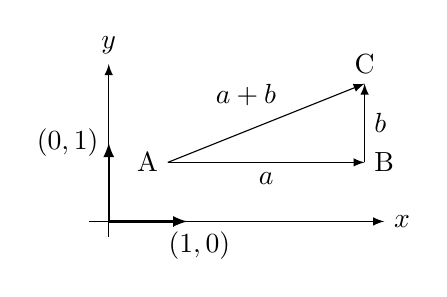
\begin{tikzpicture}
\pgfmathsetmacro{\a}{2.5}
\pgfmathsetmacro{\b}{1}
\draw[-latex](-0.25,0)--(3.5,0)node[right]{$x$};
\draw[-latex](0,-0.2)--(0,2)node[above]{$y$};
\draw[-latex] (0.75,0.75)coordinate(kA)node[left]{A}--++(\a,0)node[pos=0.5,below]{$a\ai$}node[right]{B}coordinate(kB);
\draw[-latex](kB)--++(0,\b)node[above]{C}node[pos=0.5,right]{$b\aj$};
\draw[-latex](kA)--++(\a,\b)node[pos=0.6,above left]{$a\ai+b\aj$};
\draw[-latex,thick](0,0)--(1,0)node[below,xshift={1ex}]{$(1,0)$}node[pos=0.5,below]{$\ai$};
\draw[-latex,thick](0,0)--(0,1)node[left]{$(0,1)$}node[pos=0.5,left]{$\aj$};
\end{tikzpicture}
\caption{اساس سمتیات \عددی{\ai} اور \عددی{\aj} کو استعمال کر کے کسی بھی سمتیہ \عددی{\krightharpoonup{AC}} کو لکھا جا سکتا ہے۔}
\label{شکل_سمتیہ_اساسی}
\end{minipage}\hfill
\begin{minipage}{0.45\textwidth}
\centering
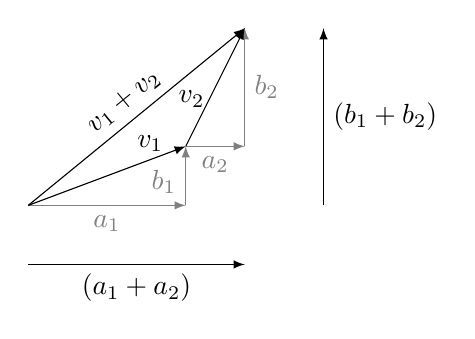
\begin{tikzpicture}
\pgfmathsetmacro{\a}{2}
\pgfmathsetmacro{\b}{0.75}
\pgfmathsetmacro{\c}{0.75}
\pgfmathsetmacro{\d}{1.5}
\draw[-latex,gray] (0,0)coordinate(kA)--++(\a,0)node[pos=0.5,below]{$a_1\ai$}coordinate(kB);
\draw[-latex,gray](kB)--++(0,\b)coordinate(kC)node[pos=0.4,left]{$b_1\aj$};
\draw[-latex](kA)--++(\a,\b)node[pos=0.85,shift={(-1ex,1ex)}]{$\kvec{v}_1$};
\draw[-latex,gray] (kC)coordinate(kAA)--++(\c,0)node[pos=0.5,below]{$a_2\ai$}coordinate(kBB);
\draw[-latex,gray](kBB)--++(0,\d)node[pos=0.5,right]{$b_2\aj$};
\draw[-latex](kAA)--++(\c,\d)node[pos=0.3,shift={(-1ex,1ex)}]{$\kvec{v}_2$}coordinate(kCC);
\draw[-latex](kA)--(kCC)node[pos=0.5,sloped,above]{$\kvec{v}_1+\kvec{v}_2$};
\draw[-latex](0,-0.75)--++(\a+\c,0)node[pos=0.5,below]{$(a_1+a_2)\ai$};
\draw[-latex](\a+\c+1,0)--++(0,\b+\d)node[pos=0.5,right]{$(b_1+b_2)\aj$};
\end{tikzpicture}
\caption{سمتیات کا مجموعہ ان کے مطابقتی اجزاء کے مجموعہ لے کر حاصل ہو گا۔}
\label{شکل_سمتیات_مجموعی_اجزاء}
\end{minipage}
\end{figure}

\ابتدا{تعریف}
اگر \عددی{\kvec{v}=a\ai+b\aj} ہو تب \عددی{\ai} اور \عددی{\aj} کے رخ، سمتیہ \عددی{\kvec{v}} کے اجزاء  سمتیات \عددی{a\ai} اور \عددی{b\aj} ہوں گے۔ اعداد \عددی{a} اور \عددی{b}، اساسی سمتیات \عددی{\ai} اور \عددی{\aj} کے رخ، سمتیہ \عددی{\kvec{v}} کے غیر سمتی اجزاء ہوں گے۔ 
\انتہا{تعریف}
%================

\ابتدا{تعریف}
سمتیات کی برابری یا یکسانیت (الجبرائی تعریف)۔
\begin{align}
a\ai+b\aj=a'\ai+b'\aj\quad \Leftrightarrow\quad a=a',\quad b=b'
\end{align}
\انتہا{تعریف}
%=======

دو سمتیات صرف اور صرف اس صورت ایک دوسرے کے برابر ہوں گے جب \عددی{\ai} اور \عددی{\aj} کے رخ، ان کے مطابقتی غیر سمتی اجزاء ایک دوسرے کے برابر ہوں۔

\جزوحصہء{الجبرائی مجموعہ}
سمتیات کے مطابقتی غیر سمتی اجزاء کا مجموعہ لے کر ان سمتیات  کا مجموعہ حاصل کیا جا سکتا ہے (شکل \حوالہ{شکل_سمتیات_مجموعی_اجزاء})۔

اگر \عددی{\kvec{v}_1=a_1\ai+b_1\aj} اور \عددی{\kvec{v}_2=a_2\ai+b_2\aj} ہوں تب درج ذیل ہو گا۔ 
\begin{align*}
\kvec{v}_1+\kvec{v}_2=(a_1+a_2)\ai+(b_1+b_2)\aj
\end{align*}

\ابتدا{مثال}
\begin{align*}
(2\ai-4\aj)+(5\ai+3\aj)=(2+5)\ai+(-4+3)\aj=7\ai-\aj
\end{align*}
\انتہا{مثال}

\begin{figure}
\centering
\begin{subfigure}{0.30\textwidth}
\centering
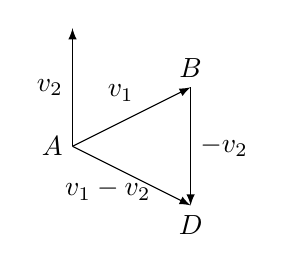
\begin{tikzpicture}
\pgfmathsetmacro{\a}{1.5}
\pgfmathsetmacro{\b}{0.75}
\pgfmathsetmacro{\aa}{0}
\pgfmathsetmacro{\bb}{1.5}
\draw[-latex](0,0)node[left]{$A$}--++(\a,\b)node[pos=0.6,above left]{$\kvec{v}_1$}node[above]{$B$}coordinate(kB);
\draw[-latex](0,0)--++(\aa,\bb)node[pos=0.5,left]{$\kvec{v}_2$};
\draw[-latex](kB)--++(\aa,-\bb)node[pos=0.5,right]{$-\kvec{v}_2$}coordinate(kD)node[below]{$D$};
\draw[-latex](0,0)--(kD)node[pos=0.4,below,xshift={-1ex}]{$\kvec{v}_1-\kvec{v}_2$};
\end{tikzpicture}
\caption{}
\end{subfigure}\hfill
\begin{subfigure}{0.30\textwidth}
\centering
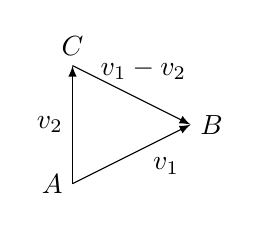
\begin{tikzpicture}
\pgfmathsetmacro{\a}{1.5}
\pgfmathsetmacro{\b}{0.75}
\pgfmathsetmacro{\aa}{0}
\pgfmathsetmacro{\bb}{1.5}
\draw[-latex](0,0)node[left]{$A$}--++(\a,\b)node[right]{$B$}node[pos=0.6,below right]{$\kvec{v}_1$}coordinate(kB);
\draw[-latex](0,0)--++(\aa,\bb)node[above]{$C$}node[pos=0.5,left]{$\kvec{v}_2$}coordinate(kC);
\draw[-latex](kC)--(kB)node[pos=0.6,above,yshift={1ex}]{$\kvec{v}_1-\kvec{v}_2$};
\end{tikzpicture}
\caption{}
\end{subfigure}\hfill
\begin{subfigure}{0.30\textwidth}
\centering
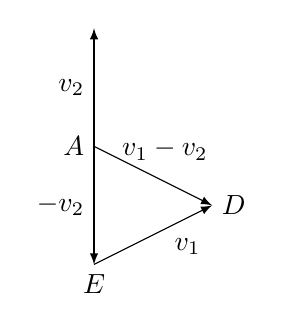
\begin{tikzpicture}
\pgfmathsetmacro{\a}{1.5}
\pgfmathsetmacro{\b}{0.75}
\pgfmathsetmacro{\aa}{0}
\pgfmathsetmacro{\bb}{1.5}
\draw[-latex](0,0)node[below]{$E$}--++(\a,\b)node[right]{$D$}node[pos=0.6,below right]{$\kvec{v}_1$}coordinate(kD);
\draw[latex-](0,0)--++(\aa,\bb)node[left]{$A$}node[pos=0.5,left]{$-\kvec{v}_2$}coordinate(kA);
\draw[-latex](kA)--(kD)node[pos=0.6,above,yshift={1ex}]{$\kvec{v}_1-\kvec{v}_2$};
\draw[-latex](kA)--++(\aa,\bb)node[pos=0.5,left]{$\kvec{v}_2$};
\end{tikzpicture}
\caption{}
\end{subfigure}
\caption{سمتیہ \عددی{\kvec{v}_1-\kvec{v}_2} کو ترسیم کرنے کے کئی طریقوں میں سے تین طریقے۔}
\label{شکل_سمتیہ_تفریق_طریقے}
\end{figure}

\جزوحصہء{تفریق}
ایک سمتیہ \عددی{\kvec{v}} کا منفی سمتیہ \عددی{-\kvec{v}=(-1)\kvec{v}} ہو گا۔ اس کی لمبائی \عددی{\kvec{v}} کی لمبائی ہو گی البتہ اس کا رخ \عددی{\kvec{v}} کا مخالف ہو گا۔سمتیہ \عددی{\kvec{v}_2} کو سمتیہ \عددی{\kvec{v}_1} سے منفی کرنے کی خاطر ہم  \عددی{-\kvec{v}_2} اور \عددی{\kvec{v}_1} کا مجموعہ لیں گے۔ جیومیٹریائی طور پر ہم \عددی{\kvec{v}_1} کے سر سے \عددی{-\kvec{v}_2} کھینچ کر \عددی{\kvec{v}_1} کے دم سے \عددی{-\kvec{v}_2} کے سر تک سمتیہ ترسیم کریں گے۔ یہ عمل شکل \حوالہ{شکل_سمتیہ_تفریق_طریقے}-ا میں دکھایا گیا ہے جہاں 
\begin{align*}
\krightharpoonup{AD}=\krightharpoonup{AB}+\krightharpoonup{BD}=\kvec{v}_1+(-\kvec{v}_2)=\kvec{v}_1-\kvec{v}_2
\end{align*}

اس کے علاوہ  \عددی{\kvec{v}_1} اور \عددی{\kvec{v}_2} کے دم مشترکہ  نقطہ پر رکھ  کر \عددی{\kvec{v}_1} اور \عددی{\kvec{v}_2} ترسیم کر کے \عددی{\kvec{v}_2} کے سر سے \عددی{\kvec{v}_1} کے سر تک سمتیہ \عددی{\kvec{v}_1-\kvec{v}_2} ہو گا۔ یہ عمل  شکل \حوالہ{شکل_سمتیہ_تفریق_طریقے}-ب میں پیش  کیا گیا ہے جہاں درج ذیل ہے۔
 \begin{align*}
\krightharpoonup{CB}=\krightharpoonup{CA}+\krightharpoonup{AB}=-\kvec{v}_2+\kvec{v}_1=\kvec{v}_1-\kvec{v}_2
\end{align*}
مزید، \عددی{-\kvec{v}_2} کے سر سے \عددی{\kvec{v}_1} ترسیم کر کے \عددی{\kvec{v}_1-\kvec{v}_2} حاصل کیا جا سکتا ہے (شکل \حوالہ{شکل_سمتیہ_تفریق_طریقے}-ج)۔

درج ذیل قاعدہ سمتیات کی تفریق کو اجزاء کی صورت میں پیش کرتا ہے۔
\begin{align}
\kvec{v}_1-\kvec{v}_2=(a_1-a_2)\ai+(b_1-b_2)\aj
\end{align}
اس قاعدہ کے تحت دو سمتیات تفریق کرنے کی خاطر ان کے مطابقتی اجزاء تفریق کیے جائیں گے۔

\ابتدا{مثال}
\begin{align*}
(6\ai+2\aj)-(3\ai-5\aj)=(6-3)\ai+(2-(-5))\aj=3\ai+7\aj
\end{align*}
\انتہا{مثال}
%============================

ہم نقطہ \عددی{N_1(x_1,y_1)} سے نقطہ \عددی{N_2(x_2,y_2)} تک سمتیہ کے اجزاء حاصل کرنے کے لئے \عددی{\krightharpoonup{ON_1}=x_1\ai+y_1\aj} کے اجزاء کو \عددی{\krightharpoonup{ON_2}=x_2\ai+y_2\aj} کے اجزاء سے منفی کرتے ہیں۔

\عددی{N_1(x_1,y_1)} سے \عددی{N_2(x_2,y_2)} تک سمتیہ درج ذیل ہو گا۔
\begin{align}
\krightharpoonup{N_1N_2}=(x_2-x_1)\ai+(y_2-y_1)\aj
\end{align}

\begin{figure}
\centering
\begin{minipage}{0.55\textwidth}
\centering
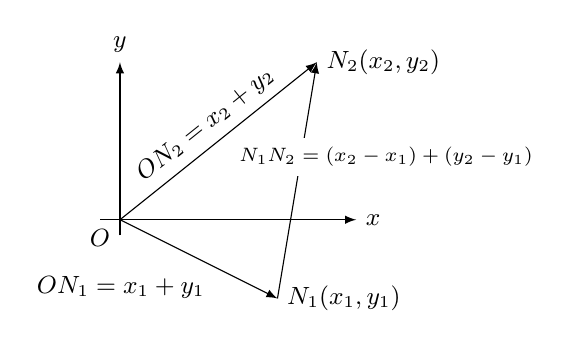
\begin{tikzpicture}[font=\small]
\pgfmathsetmacro{\a}{2}
\pgfmathsetmacro{\b}{-1}
\pgfmathsetmacro{\aa}{2.5}
\pgfmathsetmacro{\bb}{2}
\draw[-latex](-0.25,0)--(3,0)node[right]{$x$};
\draw[-latex](0,-0.2)--(0,2)node[above]{$y$};
\draw[-latex](0,0)node[below left]{$O$}--++(\a,\b)node[pos=0.6,below left]{$\krightharpoonup{ON_1}=x_1\ai+y_1\aj$}node[right]{$N_1(x_1,y_1)$}coordinate(kA);
\draw[-latex](0,0)--++(\aa,\bb)node[pos=0.5,sloped, above]{$\krightharpoonup{ON_2}=x_2\ai+y_2\aj$}node[right]{$N_2(x_2,y_2)$}coordinate(kB);
\draw[-latex](kA)--(kB)node[pos=0.6,fill=white,right,xshift=-6ex,font=\scriptsize]{$\krightharpoonup{N_1N_2}=(x_2-x_1)\ai+(y_2-y_1)\aj$};
\end{tikzpicture}
\caption{}
\end{minipage}\hfill
\begin{minipage}{0.35\textwidth}
\centering
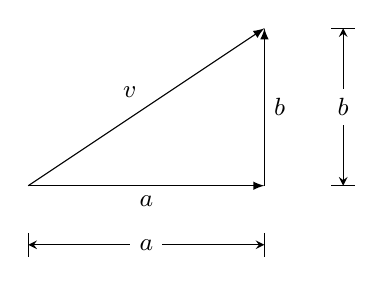
\begin{tikzpicture}[font=\small]
\pgfmathsetmacro{\a}{3}
\pgfmathsetmacro{\b}{2}
\draw[-latex](0,0)--++(\a,0)node[pos=0.5,below]{$a\ai$}coordinate(kA);
\draw[-latex](kA)--++(0,\b)node[pos=0.5,right]{$b\aj$}coordinate(kB);
\draw[-latex](0,0)--(kB)node[pos=0.5,above left]{$\kvec{v}$};
\draw[stealth-stealth](0,-0.75)--++(\a,0)node[pos=0.5,fill=white]{$\abs{a}$};
\draw[stealth-stealth](\a+1,0)--++(0,\b)node[pos=0.5,fill=white]{$\abs{b}$};
\draw(0,-0.6)--++(0,-0.3);
\draw(\a,-0.6)--++(0,-0.3);
\draw(\a+0.85,0)--++(0.3,0);
\draw(\a+0.85,\b)--++(0.3,0);
\end{tikzpicture}
\caption{سمتیہ کی لمبائی مسئلہ فیثاغورث سے حاصل کی جا سکتی ہے۔}
\label{شکل_سمتیہ_کی_لمبائی}
\end{minipage}
\end{figure}
\ابتدا{مثال}
نقطہ \عددی{N_1(3,4)} سے نقطہ \عددی{N_2(5,1)} تک سمتیہ درج ذیل ہے۔
\begin{align*}
\krightharpoonup{N_1N_2}=(5-3)\ai+(1-4)\aj=2\ai-3\aj
\end{align*}
\انتہا{مثال}
%===============

\جزوحصہء{مقدار}
سمتیہ \عددی{\kvec{v}=a\ai+b\aj} کی \اصطلاح{لمبائی}\فرہنگ{سمتیہ!لمبائی}\حاشیہب{length}\فرہنگ{vector!length} یا \اصطلاح{مقدار}\فرہنگ{سمتیہ!مقدار}\حاشیہب{magnitude}\فرہنگ{vector!magnitude} \عددی{\abs{\kvec{v}}=\sqrt{a^2+b^2}} ہے۔  سمتیہ \عددی{\kvec{v}} اور اس کے دو سمتیہ اجزاء کے قائمہ مثلث پر مسئلہ فیثاغورث لاگو کرنے سے یہ کلیہ اخذ ہوتا ہے (شکل \حوالہ{شکل_سمتیہ_کی_لمبائی})۔ سمتیہ کی لمبائی \عددی{\abs{\kvec{v}}} میں دو انتصابی لکیریں وہی ہیں جو مطلق قیمت کو ظاہر کرنے کے لئے استعمال کی جاتی ہیں۔ 

\begin{align}
\abs{\kvec{v}}&=\sqrt{a^2+b^2}&&\kvec{v}=a\ai+b\aj
\end{align}

\ابتدا{مثال}\شناخت{مثال_سمتیہ_ہاتھ_ریڑھی}
آپ زمین کے ساتھ \عددی{30^{\circ}} زاویہ پر \عددی{\SI{20}{\newton}} کی قوت \عددی{\kvec{F}} سے ہاتھ ریڑھی کو دکھا لگاتے ہیں (شکل \حوالہ{شکل_مثال_سمتیہ_ہاتھ_ریڑھی}-ا)۔ قوت کا افقی جزو ریڑھی کو حرکت دیتا ہے جبکہ اس کا انتصابی جزو ریڑھی کا وزن بڑھاتا ہے۔ اس قوت کا افقی اور انتصابی جزو معلوم کریں۔

حل:\quad
ہم قوت \عددی{\kvec{F}=a\ai+b\aj} اور اس کے اجزاء کے لئے مثلث  بناتے ہیں (شکل \حوالہ{شکل_مثال_سمتیہ_ہاتھ_ریڑھی}-ب اور شکل \حوالہ{شکل_مثال_سمتیہ_ہاتھ_ریڑھی}-ج)۔ اس مثلث سے \عددی{a=10\sqrt{3}} اور \عددی{b=10} حاصل ہوتے ہیں۔ قوت کا افقی جزو \عددی{10\sqrt{3}\ai} اور انتصابی جزو \عددی{-10\aj} ہے۔یوں \عددی{\kvec{F}=10\sqrt{3}\ai-10\aj} ہو گا۔  انتصابی جزو کا رخ نیچے ہے لہٰذا یہ منفی ہے۔ 
\انتہا{مثال}
%==================
\begin{figure}
\centering
\begin{subfigure}{0.30\textwidth}
\centering
\begin{tikzpicture}
\pgfmathsetmacro{\kx}{1.5}
\pgfmathsetmacro{\ky}{0.5}
\pgfmathsetmacro{\r}{0.1}
\pgfmathsetmacro{\len}{2}
\pgfmathsetmacro{\ang}{150}
\draw(0,0)--++(\kx,0)--++(0,-\ky)--++(-\kx,0)--++(0,\ky);
\draw(1/2*\kx,-1/2*\ky)node[]{\RL{ہاتھ ریڑھی}};
\draw([shift={(180:\r)}]1/4*\kx,-\ky) arc (180:360:\r);
\draw([shift={(180:\r)}]3/4*\kx,-\ky) arc (180:360:\r);
\draw[latex-](0,0)--++(\ang:\len)node[pos=0.5,above right]{$\abs{\kvec{F}}=20$};
\draw[dashed](0,0)--(-2,0);
\draw[]([shift={(\ang:0.5)}]0,0) arc (\ang:180:0.5)node[pos=0.3,left]{$30^{\circ}$};
\end{tikzpicture}
\caption{}
\end{subfigure}\hfill
\begin{subfigure}{0.30\textwidth}
\centering
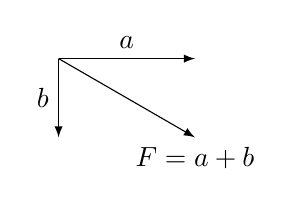
\begin{tikzpicture}
\pgfmathsetmacro{\len}{2}
\pgfmathsetmacro{\ang}{150}
\pgfmathsetmacro{\a}{\len*cos(180-\ang)}
\pgfmathsetmacro{\b}{\len*sin(\ang)}
\draw[-latex](0,0)--(\a,0)node[pos=0.5,above]{$a\ai$};
\draw[-latex](0,0)--(0,-\b)node[pos=0.5,left]{$b\aj$};
\draw[-latex](0,0)--++(\ang-180:\len)node[below]{$\kvec{F}=a\ai+b\aj$};
\end{tikzpicture}
\caption{}
\end{subfigure}\hfill
\begin{subfigure}{0.30\textwidth}
\centering
\begin{tikzpicture}[font=\small]
\pgfmathsetmacro{\len}{2}
\pgfmathsetmacro{\ang}{150}
\pgfmathsetmacro{\a}{\len*cos(180-\ang)}
\pgfmathsetmacro{\b}{\len*sin(\ang)}
\draw[](0,-\b)--++(\a,0)node[pos=0.5,below]{$\abs{a\ai}=a$};
\draw[](0,0)--(0,-\b)node[below left]{$B$}node[pos=0.5,left]{$\abs{b\aj}=b$};
\draw[](0,0)node[above]{$A$}--++(\ang-180:\len)node[below right]{$C$}node[pos=0.3,above right]{$\abs{\kvec{F}}=20$};
\draw([shift={(270:0.3)}]0,0) arc (270:330:0.3)node[pos=0.6,below]{$\tfrac{\pi}{3}$};
\draw([shift={(\ang:0.6)}]\a,-\b) arc (\ang:180:0.6)node[pos=0.35,left]{$\tfrac{\pi}{6}$};
\end{tikzpicture}
\caption{}
\end{subfigure}
\caption{ہاتھ ریڑھی (مثال \حوالہ{مثال_سمتیہ_ہاتھ_ریڑھی})}
\label{شکل_مثال_سمتیہ_ہاتھ_ریڑھی}
\end{figure}
\جزوحصہء{غیر سمتی ضرب}
غیر سمتی ضرب جزو در جزو حاصل کیا جا سکتا ہے۔ اگر \عددی{c} ایک غیر سمتی اور \عددی{\kvec{v}=a\ai+b\aj} ایک سمتیہ ہو تب درج ذیل ہو گا۔
\begin{align}
c\kvec{v}=c(a\ai+b\aj)=(ca)\ai+(cb)\aj
\end{align}
سمتیہ \عددی{c\kvec{v}} کی لمبائی سمتیہ \عددی{\kvec{v}} کی لمبائی ضرب \عددی{\abs{c}} ہو گا:
\begin{align*}
\abs{c\kvec{v}}&=\abs{(ca)\ai+(cb)\aj}\\
&=\sqrt{(ca)^2+(cb)^2}\\
&=\sqrt{c^2(a^2+b^2)}\\
&=\sqrt{c^2}\sqrt{a^2+b^2}\\
&=\abs{c}\abs{\kvec{v}}
\end{align*}

یوں اگر \عددی{c} غیر سمتی ہو اور \عددی{\kvec{v}} ایک سمتیہ ہو تب \عددی{\abs{c\kvec{v}}=\abs{c}\abs{\kvec{v}}} ہو گا۔

\ابتدا{مثال}
اگر \عددی{c=-2} اور \عددی{\kvec{v}=-3\ai+4\aj} ہوں تب درج ذیل ہو گا۔
\begin{align*}
\abs{\kvec{v}}&=\abs{-3\ai+4\aj}=\sqrt{(-3)^2+(4)^2}=\sqrt{9+16}=\sqrt{25}=5\\
\abs{-2\kvec{v}}&=\abs{(-2)(-3\ai+4\aj)}=\abs{6\ai-8\aj}=\sqrt{(6)^2+(-8)^2}\\
&=\sqrt{36+64}=\sqrt{100}=10=\abs{-2}\abs{5}=\abs{c}\abs{\kvec{v}}
\end{align*}
\انتہا{مثال}
%======================

\جزوحصہء{صفر سمتیہ}
صفر سمتیہ سے مراد درج ذیل سمتیہ ہے۔
\begin{align*}
\kvec{0}=0\ai+0\aj
\end{align*}
دھیان رہے کہ صفر سمتیہ \عددی{\kvec{0}} کو ظاہر کرنے کے لئے \عددی{0} کو موٹی لکھائی میں لکھا جاتا ہے۔صفر سمتیہ وہ واحد سمتیہ ہے جس کی لمبائی صفر ہے۔ یہ حقیقت درج ذیل سے واضح ہے۔
\begin{align*}
\abs{a\ai+b\aj}=\sqrt{a^2+b^2}=0\quad \Leftrightarrow\quad a=b=0
\end{align*}

\begin{figure}
\centering
\begin{tikzpicture}[font=\small]
\pgfmathsetmacro{\r}{1.5}
\pgfmathsetmacro{\ang}{40}
\pgfmathsetmacro{\a}{\r*cos(\ang)}
\pgfmathsetmacro{\b}{\r*sin(\ang)}
\draw[-latex](-1.25*\r,0)--(1.75*\r,0)node[right]{$x$};
\draw[-latex](0,-1.1*\r)--(0,1.5*\r)node[above]{$y$};
\draw(0,0) circle (\r);
\draw[-latex,thick](0,0)--(\r,0)node[below right]{$(1,0)$};
\draw[-latex,thick](0,0)--(0,\r)node[above left]{$(0,1)$}node[pos=0.5,left]{$\aj$};
\draw[-latex,thick](0,0)--++(\ang:\r)node[pos=0.65,above]{$\kvec{u}$};
\draw[-latex,thick](0,0)--++(\a,0)node[pos=0.5,below]{$(\cos\theta)\ai$};
\draw[-latex,thick](\a,0)--++(0,\b)node[pos=0.5,right,fill=white]{$(\sin\theta)\aj$};
\draw[-stealth]([shift={(0:0.5)}]0,0) arc (0:\ang:0.5)node[pos=0.6,right]{$\theta$};
\draw(135:\r)node[pin=135:{\RL{اکائی دائرہ}}]{};
\end{tikzpicture}
\caption{مستوی میں ہر اکائی سمتیہ کو \عددی{\kvec{u}=(\cos\theta)\ai+(\sin\theta)\aj} روپ میں لکھا جا سکتا ہے۔}
\label{شکل_سمتیہ_اکائی_دائرہ}
\end{figure}
\جزوحصہء{اکائی سمتیات}
کوئی بھی سمتیہ جس کی لمبائی \عددی{1} ہو \اصطلاح{اکائی سمتیہ}\فرہنگ{سمتیہ!اکائی}\حاشیہب{unit vector}\فرہنگ{vector!unit} کہلائے گا۔ سمتیات \عددی{\ai} اور \عددی{\aj} اکائی سمتیات ہیں۔
\begin{align*}
\abs{\ai}=\abs{1\ai+0\aj}=\sqrt{1^2+0^2}=1,\quad \abs{\aj}=\abs{0\ai+1\aj}=\sqrt{0^2+1^2}=1
\end{align*}

سمتیہ \عددی{\kvec{u}} جو اکائی سمتیہ \عددی{\ai} کو  \عددی{\theta} زاویہ مثبت رخ گھما کر حاصل ہو گا،  کے سمتی اجزاء درج ذیل ہوں گے (شکل \حوالہ{شکل_سمتیہ_اکائی_دائرہ})۔
\begin{align}
\kvec{u}=(\cos\theta)\ai+(\sin\theta)\aj
\end{align}
چونکہ اکائی سمتیہ کو گھمانے سے اس کی لمبائی تبدیل نہیں ہوتی لہٰذا \عددی{\kvec{u}} بھی اکائی سمتیہ ہو گا یعنی:
\begin{align*}
\abs{\kvec{u}}=\sqrt{(\cos\theta)^2+(\sin\theta)^2}=\sqrt{1^2}=1
\end{align*}
زاویہ \عددی{\theta} کو \عددی{0} تا \عددی{2\pi} کرنے سے \عددی{\kvec{u}} کا سر \عددی{N} مبدا کے گرد، گھڑی کے الٹ رخ،  دائرہ \عددی{x^2+y^2=1} پر چلتا ہے جو مستوی میں ہر ممکنہ رخ  کا اکائی سمتیہ دے گا۔

\جزوحصہء{لمبائی اور رخ}
اگر \عددی{\kvec{v}\ne \kvec{0}} ہو تب
\begin{align*}
\abs{\frac{\kvec{v}}{\abs{\kvec{v}}}}=\abs{\frac{1}{\abs{\kvec{v}}}\kvec{v}}=\frac{1}{\abs{\kvec{v}}}\abs{\kvec{v}}=1
\end{align*}
ہو گا لہٰذا \عددی{\tfrac{\kvec{v}}{\abs{\kvec{v}}}} اکائی سمتیہ ہو گا جس کا رخ \عددی{\kvec{v}} کا رخ ہو گا۔یوں ہم \عددی{\kvec{v}} کو اس کی دو اہم خواص، لمبائی اور رخ، کی صورت میں درج ذیل لکھ سکتے ہیں۔
\begin{align*}
\kvec{v}=\abs{\kvec{v}}\big(\tfrac{\kvec{v}}{\abs{\kvec{v}}}\big)
\end{align*}

یوں اگر \عددی{\kvec{u}\ne \kvec{0}} ہو تب
\begin{enumerate}[a.]
\item
\عددی{\tfrac{\kvec{v}}{\abs{\kvec{v}}}} اکائی سمتیہ ہو گا جس کا رخ \عددی{\kvec{v}} کا رخ ہو گا۔ یوں ہم \عددی{\tfrac{\kvec{v}}{\abs{\kvec{v}}}} کو \عددی{\kvec{v}} کو رخ کہتے ہیں۔
\item
مساوات \عددی{\kvec{v}=\abs{\kvec{v}}(\tfrac{\kvec{v}}{\abs{\kvec{v}}})} سمتیہ \عددی{\kvec{v}} کو اس کی لمبائی اور رخ کی صورت میں  بیان کرتی ہے۔
\end{enumerate}

\ابتدا{مثال}
سمتیہ \عددی{\kvec{v}=3\ai-4\aj} کو اس کی لمبائی اور رخ کا حاصل ضرب لکھیں۔
 
حل:\quad
\begin{align*}
\abs{\kvec{v}}&=\sqrt{(3)^2+(-4)^2}=\sqrt{9+16}=5&&\text{\RL{\عددی{\kvec{v}} کی لمبائی}}\\
\frac{\kvec{v}}{\abs{\kvec{v}}}&=\frac{3\ai-4\aj}{5}=\frac{3}{5}\ai-\frac{4}{5}\aj&&\text{\RL{\عددی{\kvec{v}} کا رخ}}\\
\kvec{v}&=3\ai-4\aj=\underbrace{5}_{\text{لمبائی}}\big(\underbrace{\frac{3}{5}\ai-\frac{4}{5}\aj}_{\text{رخ}}\big)
\end{align*}
\انتہا{مثال}
%====================

\جزوحصہء{ڈھلوان، مماس اور عمود}
ایک سمتیہ اس صورت ایک خط کے متوازی ہو گا جب سمتیہ کو ظاہر کرنے والا قطع اور یہ خط متوازی ہوں۔ ایک غیر انتصابی سمتیہ کی ڈھلوان ان خطوط کی ڈھلوان ہو گی جو اس سمتیہ کے متوازی ہوں۔ یوں \عددی{a\ne 0} کی صورت میں سمتیہ \عددی{\kvec{v}=a\ai+b\aj} کا ڈھلوان \عددی{\tfrac{b}{a}} ہو گا (شکل \حوالہ{شکل_سمتیہ_ڈھلوان_تعریف})۔

کسی نقطہ پر ایک منحنی کو ایک سمتیہ تب \اصطلاح{مماسی}\فرہنگ{مماس}\حاشیہب{tangent}\فرہنگ{tangent} یا \اصطلاح{عمودی}\فرہنگ{عمودی}\حاشیہب{normal}\فرہنگ{normal} ہو گا جب اس نقطہ پر منحنی کا مماس  اور یہ سمتیہ متوازی یا عمودی ہوں۔ اگلی مثال میں ایسی سمتیہ کو تلاش کرنا دکھایا گیا ہے۔
\begin{figure}
\centering
\begin{minipage}{0.45\textwidth}
\centering
\begin{tikzpicture}
\pgfmathsetmacro{\a}{3}
\pgfmathsetmacro{\b}{2}
\pgfmathsetmacro{\ang}{atan(\b/\a)}
\draw[-latex](0,0)--++(\a,0)node[pos=0.5,below]{$a\ai$};
\draw[-latex](\a,0)--++(0,\b)node[pos=0.5,right]{$b\aj$};
\draw[-latex](0,0)--(\a,\b)node[pos=0.5,left,xshift={-0.5ex}]{$a\ai+b\aj$};
\draw(\ang:2.5)node[pin=135:{ڈھلوان\,\عددی{\tfrac{b}{a}}}]{};
\draw[-stealth]([shift={(0:0.6)}]0,0) arc (0:\ang:0.6)node[pos=0.6,right]{$\theta$};
\end{tikzpicture}
\caption{اگر \عددی{a\ne 0} ہو تب سمتیہ \عددی{\kvec{v}=a\ai+b\aj} کی ڈھلوان \عددی{\tfrac{b}{a}} ہو گی۔}
\label{شکل_سمتیہ_ڈھلوان_تعریف}
\end{minipage}\hfill
\begin{minipage}{0.45\textwidth}
\centering
\begin{tikzpicture}[declare function={f(\x)=1/2*\x^3+1/2;}]
\begin{axis}[clip=false,small,axis equal,axis lines=middle,ymin=0,xlabel={$x$},ylabel={$y$},xlabel style={at={(current axis.right of origin)},anchor=west},ylabel style={at={(current axis.above origin)},anchor=south},xtick={1},ytick={1}]
\addplot[domain=0:1.5] {f(x)}node[above]{$y=\tfrac{x^3}{2}+\tfrac{1}{2}$};
\draw[-stealth](axis cs:1,1)--(axis cs:{1+2/sqrt(13)},{1+3/sqrt(13)})coordinate(ka)node[pos=0.5,right]{$\kvec{u}=\tfrac{2}{\sqrt{13}}\ai+\tfrac{3}{\sqrt{13}}\aj$};
\draw[-stealth](axis cs:1,1)--(axis cs:{1-2/sqrt(13)},{1-3/sqrt(13)})node[pos=0.5,right]{$-\kvec{u}$};
\draw[-stealth](axis cs:1,1)--(axis cs:{1-3/sqrt(13)},{1+2/sqrt(13)})node[above]{$\kvec{n}=-\tfrac{3}{\sqrt{13}}\ai+\tfrac{2}{\sqrt{13}}\aj$};
\draw[-stealth](axis cs:1,1)--(axis cs:{1+3/sqrt(13)},{1-2/sqrt(13)})coordinate(kb)node[pos=0.5,above]{$-\kvec{n}$};
\RightAngle{({1+2/sqrt(13)},{1+3/sqrt(13)})}{(1,1)}{({1+3/sqrt(13)},{1-2/sqrt(13)})}
\end{axis}
\end{tikzpicture}
\caption{ایک نقطہ پر ترسیم کا اکائی مماسی اور اکائی عمودی سمتیہ (مثال \حوالہ{مثال_سمتیہ_مماس_عمود})}
\label{شکل_مثال_سمتیہ_مماس_عمود}
\end{minipage}
\end{figure}
\ابتدا{مثال}\شناخت{مثال_سمتیہ_مماس_عمود}
نقطہ \عددی{(1,1)} پر منحنی \عددی{y=\tfrac{x^3}{2}+\tfrac{1}{2}} کو مماسی اور عمودی اکائی سمتیات تلاش کریں۔

حل:\quad
ہم نقطہ \عددی{(1,0)} پر منحنی کے مماس کے متوازی اور عمودی اکائی سمتیات معلوم کرتے ہیں (شکل \حوالہ{شکل_مثال_سمتیہ_مماس_عمود})۔

اس نقطہ پر منحنی کے مماس کی ڈھلوان درج ذیل ہو گی۔
\begin{align*}
y'=\left.\frac{3x^2}{2}\right\vert_{x=1}=\frac{3}{2}
\end{align*}
ہم اتنی ڈھلوان کی اکائی سمتیہ تلاش کرتے ہیں۔ سمتیہ \عددی{\kvec{v}=2\ai+3\aj} اور اس کے ہر غیر صفر مضرب کی ڈھلوان \عددی{\tfrac{3}{2}} ہے۔ سمتیہ  \عددی{\kvec{v}} کا ایسا مضرب معلوم کرنے کے لئے جس کی لمبائی \عددی{1} ہو ہم \عددی{\kvec{v}} کو 
\begin{align*}
\abs{\kvec{v}}=\sqrt{2^2+3^2}=\sqrt{13}
\end{align*}
سے تقسیم کرتے ہیں۔ یوں درج ذیل حاصل ہو گا۔
\begin{align*}
\kvec{u}=\frac{\kvec{v}}{\abs{\kvec{v}}}=\frac{2}{\sqrt{13}}\ai+\frac{3}{\sqrt{13}}\aj
\end{align*}
سمتیہ \عددی{\kvec{u}} کی لمبائی \عددی{1} ہے اور یہ \عددی{(1,1)} پر منحنی کا مماس ہے۔ درج ذیل سمتیہ
\begin{align*}
-\kvec{u}=-\frac{2}{\sqrt{13}}\ai-\frac{3}{\sqrt{13}}\aj
\end{align*}
جو مخالف  رخ ہے بھی \عددی{(1,1)} پر منحنی کا مماس ہو گا۔ کسی اضافی شرط کے بغیر ان میں سے کسی ایک اکائی مماسی سمتیہ کو دوسری اکائی مماسی سمتیہ پر فوقیت نہیں دی جا سکتی ہے۔

نقطہ \عددی{(1,1)} پر منحنی کا عمودی سمتیہ تلاش کرنے کی خاطر ہم ایسا اکائی سمتیہ معلوم کرتے ہیں جس کی ڈھلوان \عددی{\kvec{u}} کی ڈھلوان کے بالعکس متناسب کے منفی کے برابر ہو۔ ہم \عددی{\kvec{u}} کے غیر سمتی اجزاء کے مقامات آپس میں تبدیل کر کے اور ان میں سے کسی ایک کی علامت بدل کر ایسا سمتیہ معلوم کر سکتے ہیں۔ یوں درج ذیل حاصل ہو گا۔
\begin{align*}
\kvec{n}=-\frac{3}{\sqrt{13}}\ai+\frac{2}{\sqrt{13}}\aj,\quad \text{}\quad -\kvec{n}=\frac{3}{\sqrt{13}}\ai-\frac{2}{\sqrt{13}}\aj
\end{align*}  
یہاں بھی دونوں اکائی سمتیات دیے گئے نقطہ پر منحنی کو عمودی ہیں۔ ان دو عمودی اکائی سمتیات کا رخ ایک دوسرے کے الٹ ہے لیکن دونوں \عددی{(1,1)} پر منحنی کو عمودی ہیں۔
\انتہا{مثال}
%====================

\حصہء{سوالات}
\موٹا{جیومیٹری اور حساب}\\
\ابتدا{سوال}\شناخت{سوال_سمتیہ_الف}
مستوی میں پائے جانے والے سمتیات \عددی{\kvec{A}}، \عددی{\kvec{B}} اور \عددی{\kvec{C}} کو شکل \حوالہ{شکل_سوال_سمتیہ_الف} میں دکھایا گیا ہے۔ انہیں کاغذ پر اتار کر سر کے ساتھ دم جوڑ کر درج ذیل ترسیم کریں۔
\begin{multicols}{4}
\begin{enumerate}[a.]
\item
$\kvec{A}+\kvec{B}$
\item
$\kvec{A}+\kvec{B}+\kvec{C}$
\item
$\kvec{A}-2\kvec{B}$
\item
$\frac{1}{2}\kvec{A}-\kvec{C}$
\end{enumerate}
\end{multicols}
جوابات:\quad
شکل \حوالہ{شکل_سوال_سمتیہ_جوابات_چند_جمع_منفی}
\انتہا{سوال}
%=======================
\ابتدا{سوال}\شناخت{سوال_سمتیہ_ب}
مستوی میں پائے جانے والے سمتیات \عددی{\kvec{A}}، \عددی{\kvec{B}} اور \عددی{\kvec{C}} کو شکل \حوالہ{شکل_سوال_سمتیہ_ب} میں دکھایا گیا ہے۔ انہیں کاغذ پر اتار کر سر کے ساتھ دم جوڑ کر درج ذیل ترسیم کریں۔
\begin{multicols}{4}
\begin{enumerate}[a.]
\item
$\kvec{A}-\kvec{B}$
\item
$\kvec{A}+\kvec{B}+\kvec{C}$
\item
$2\kvec{A}-\frac{1}{2}\kvec{B}$
\item
$\kvec{A}-(\kvec{B}-\kvec{C})$
\end{enumerate}
\end{multicols}
\انتہا{سوال}
%=======================
\begin{figure}
\centering
\begin{minipage}{0.22\textwidth}
\centering
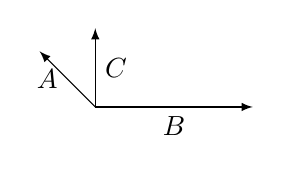
\begin{tikzpicture}
\pgfmathsetmacro{\a}{135}
\pgfmathsetmacro{\b}{1}
\pgfmathsetmacro{\aa}{0}
\pgfmathsetmacro{\bb}{2}
\pgfmathsetmacro{\aaa}{90}
\pgfmathsetmacro{\bbb}{1}
\draw[-latex](0,0)--(\a:\b)node[pos=0.5,left]{$A$};
\draw[-latex](0,0)--(\aa:\bb)node[pos=0.5,below]{$B$};
\draw[-latex](0,0)--(\aaa:\bbb)node[pos=0.5,right]{$C$};
\end{tikzpicture}
\caption{}
\label{شکل_سوال_سمتیہ_الف}
\end{minipage}\hfill
\begin{minipage}{0.22\textwidth}
\centering
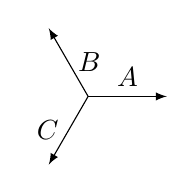
\begin{tikzpicture}
\pgfmathsetmacro{\a}{0}
\pgfmathsetmacro{\b}{1}
\pgfmathsetmacro{\aa}{120}
\pgfmathsetmacro{\bb}{1}
\pgfmathsetmacro{\aaa}{-120}
\pgfmathsetmacro{\bbb}{1}
\draw[-latex](0,0)--(\a:\b)node[pos=0.5,above]{$A$};
\draw[-latex](0,0)--(\aa:\bb)node[pos=0.5,right]{$B$};
\draw[-latex](0,0)--(\aaa:\bbb)node[pos=0.5,left]{$C$};
\end{tikzpicture}
\caption{}
\label{شکل_سوال_سمتیہ_ب}
\end{minipage}
\begin{minipage}{0.22\textwidth}
\centering
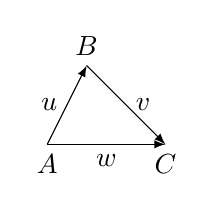
\begin{tikzpicture}
\draw[-latex](0,0)node[below]{$A$}--(1.5,0)node[pos=0.5,below]{$\kvec{w}$}node[below]{$C$};
\draw[-latex](0,0)--(0.5,1)node[pos=0.5,left]{$\kvec{u}$}node[above]{$B$};
\draw[-latex](0.5,1)--(1.5,0)node[pos=0.5,right]{$\kvec{v}$};
\end{tikzpicture}
\caption{}
\label{شکل_سوال_سمتیہ_پ}
\end{minipage}
\begin{minipage}{0.22\textwidth}
\centering
\begin{tikzpicture}
\draw[-latex](0,0)node[left]{$A$}--(2,0)node[pos=0.5,below]{$\kvec{w}$}node[right]{$C$};
\draw[-latex](0,0)--(0.5,1)node[pos=0.5,left]{$\kvec{u}$}node[above]{$B$};
\draw[-latex](0.5,1)--(2,0);
\draw[-latex](0,0)--(1.25,0.5)node[pos=0.5,above]{$\kvec{a}$}node[circ]{}node[right]{$N$};
\end{tikzpicture}
\caption{}
\label{شکل_سوال_سمتیہ_ت}
\end{minipage}
\end{figure}
%==================================================
\begin{figure}
\centering
\begin{subfigure}{0.45\textwidth}
\centering
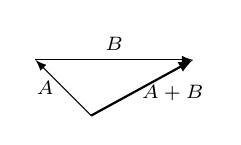
\begin{tikzpicture}[font=\scriptsize]
\pgfmathsetmacro{\a}{135}
\pgfmathsetmacro{\b}{1}
\pgfmathsetmacro{\aa}{0}
\pgfmathsetmacro{\bb}{2}
\pgfmathsetmacro{\aaa}{90}
\pgfmathsetmacro{\bbb}{1}
\draw[-latex](0,0)--(\a:\b)node[pos=0.5,left]{$A$};
\draw[-latex](\a:\b)--++(\aa:\bb)coordinate(khead)node[pos=0.5,above]{$B$};
\draw[thick,-latex](0,0)--++(khead)node[pos=0.4,right]{$A+B$};
\end{tikzpicture}
\caption{}
\end{subfigure}\hfill
\begin{subfigure}{0.45\textwidth}
\centering
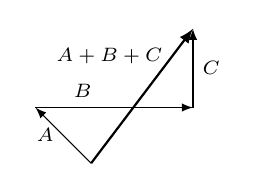
\begin{tikzpicture}[font=\scriptsize]
\pgfmathsetmacro{\a}{135}
\pgfmathsetmacro{\b}{1}
\pgfmathsetmacro{\aa}{0}
\pgfmathsetmacro{\bb}{2}
\pgfmathsetmacro{\aaa}{90}
\pgfmathsetmacro{\bbb}{1}
\draw[-latex](0,0)--(\a:\b)node[pos=0.5,left]{$A$};
\draw[-latex](\a:\b)--++(\aa:\bb)coordinate(ka)node[pos=0.3,above]{$B$};
\draw[-latex](ka)--++(\aaa:\bbb)coordinate(kb)node[pos=0.5,right]{$C$};
\draw[thick,-latex](0,0)--(kb)node[pos=0.8,left]{$A+B+C$};
\end{tikzpicture}
\caption{}
\end{subfigure}
\begin{subfigure}{0.45\textwidth}
\centering
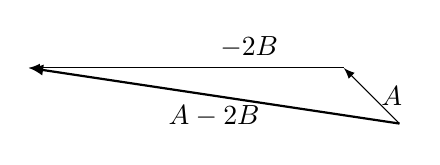
\begin{tikzpicture}
\pgfmathsetmacro{\a}{135}
\pgfmathsetmacro{\b}{1}
\pgfmathsetmacro{\aa}{0}
\pgfmathsetmacro{\bb}{2}
\pgfmathsetmacro{\aaa}{90}
\pgfmathsetmacro{\bbb}{1}
\draw[-latex](0,0)--(\a:\b)node[pos=0.5,right]{$A$};
\draw[-latex](\a:\b)--++(\aa:-2*\bb)coordinate(ka)node[pos=0.3,above]{$-2B$};
\draw[thick,-latex](0,0)--(ka)coordinate(kb)node[pos=0.5,below]{$A-2B$};
\end{tikzpicture}
\caption{}
\end{subfigure}%
\begin{subfigure}{0.45\textwidth}
\centering
\begin{tikzpicture}
\pgfmathsetmacro{\a}{135}
\pgfmathsetmacro{\b}{1}
\pgfmathsetmacro{\aa}{0}
\pgfmathsetmacro{\bb}{2}
\pgfmathsetmacro{\aaa}{90}
\pgfmathsetmacro{\bbb}{1}
\draw[-latex](0,0)--(\a:1/2*\b)node[pos=0.5,above right]{$\tfrac{1}{2}A$};
\draw[-latex](\a:1/2*\b)--++(\aaa:-\bbb)coordinate(ka)node[pos=0.3,left]{$-C$};
\draw[thick,-latex](0,0)--(ka)coordinate(kb)node[pos=0.5,right]{$\tfrac{1}{2}A-C$};
\end{tikzpicture}
\caption{}
\end{subfigure}
\caption{}
\label{شکل_سوال_سمتیہ_جوابات_چند_جمع_منفی}
\end{figure}
سوال \حوالہ{سوال_سمتیہ_مجموعات_الف} تا سوال \حوالہ{سوال_سمتیہ_مجموعات_ب} میں \عددی{\kvec{A}=2\ai-7\aj}، \عددی{\kvec{B}=\ai+6\aj} اور \عددی{\kvec{C}=\sqrt{3}\ai-\pi\aj} لیں۔ نتائج کو \عددی{a\ai+b\aj} روپ میں لکھیں۔

\ابتدا{سوال}\شناخت{سوال_سمتیہ_مجموعات_الف}
$\kvec{A}+2\kvec{B}$\\
جواب:\quad
$4\ai+5\aj$
\انتہا{سوال}
%====================
\ابتدا{سوال}
$\kvec{A}+\kvec{B}-\kvec{C}$
\انتہا{سوال}
%====================
\ابتدا{سوال}
$3\kvec{A}-\frac{1}{\pi}\kvec{C}$\\
جواب:\quad
$(6-\tfrac{\sqrt{3}}{\pi})\ai-20\aj$
\انتہا{سوال}
%====================
\ابتدا{سوال}\شناخت{سوال_سمتیہ_مجموعات_ب}
$2\kvec{A}-3\kvec{B}+32\aj$
\انتہا{سوال}
%====================
\ابتدا{سوال}\شناخت{سوال_سمتیہ_پ}
مثلث \عددی{ABC}  کے اضلاع سمتیات \عددی{\kvec{u}}، \عددی{\kvec{v}} اور \عددی{\kvec{w}} دیتے ہیں (شکل \حوالہ{شکل_سوال_سمتیہ_پ})۔
\begin{enumerate}[a.]
\item
\عددی{\kvec{w}} کو \عددی{\kvec{u}} اور \عددی{\kvec{v}} کی صورت میں لکھیں۔
\item
\عددی{\kvec{v}} کو \عددی{\kvec{u}} اور \عددی{\kvec{w}} کی صورت میں لکھیں۔
\end{enumerate}
جواب:\quad
(ا) \عددی{\kvec{w}=\kvec{v}+\kvec{u}} (ب) \عددی{\kvec{v}=\kvec{w}-\kvec{u}}
\انتہا{سوال}
%===================
\ابتدا{سوال}\شناخت{سوال_سمتیہ_ت}
مثلث \عددی{ABC} کے اضلاع  سمتیات \عددی{\kvec{u}} اور \عددی{\kvec{w}} دیتے ہیں جبکہ \عددی{BC} کا وسطی نقطہ \عددی{N} ہے (شکل \حوالہ{شکل_سوال_سمتیہ_ت})۔ سمتیہ \عددی{\kvec{a}} کو \عددی{\kvec{u}} اور \عددی{\kvec{w}} کی صورت میں لکھیں۔
\انتہا{سوال}
%==================

سوال \حوالہ{سوال_سمتیہ_نقطہ_الف} تا سوال \حوالہ{سوال_سمتیہ_نقطہ_ٹ} میں سمتیہ کو \عددی{a\ai+b\aj} روپ میں لکھیں۔ محددی سطح پر مبدا سے شروع کرتے ہوئے  انہیں ترسیم کریں۔

\ابتدا{سوال}\شناخت{سوال_سمتیہ_نقطہ_الف}
نقاط \عددی{N_1(5,7)} اور \عددی{N_2(2,9)} کے بیچ قطع \عددی{\krightharpoonup{N_1N_2}} تلاش کریں۔\\
جواب:\quad
شکل \حوالہ{شکل_سوال_سمتیہ_نقطہ_الف}
\انتہا{سوال}
%======================
\ابتدا{سوال}
نقاط \عددی{N_1(1,2)} اور \عددی{N_2(-3,5)} کے بیچ قطع \عددی{\krightharpoonup{N_1N_2}}  تلاش کریں۔
\انتہا{سوال}
%======================
\ابتدا{سوال}\شناخت{سوال_سمتیہ_نقطہ_ب}
نقاط \عددی{A(-5,3)} اور \عددی{B(-10,8)} کے بیچ قطع \عددی{\krightharpoonup{AB}}  تلاش کریں۔\\
جواب:\quad
شکل \حوالہ{شکل_سوال_سمتیہ_نقطہ_ب}
\انتہا{سوال}
%======================
\ابتدا{سوال}
نقاط \عددی{A(-7,-8)} اور \عددی{B(6,11)} کے بیچ قطع \عددی{\krightharpoonup{AB}}  تلاش کریں۔
\انتہا{سوال}
%======================
\ابتدا{سوال}\شناخت{سوال_سمتیہ_نقطہ_پ}
نقاط \عددی{N_1(1,3)} اور \عددی{N_2(2,-1)} کے بیچ قطع \عددی{\krightharpoonup{N_1N_2}}  تلاش کریں۔\\
جواب:\quad
شکل \حوالہ{شکل_سوال_سمتیہ_نقطہ_پ}
\انتہا{سوال}
%======================
\ابتدا{سوال}
نقاط \عددی{N_3(1,3)} اور \عددی{N_4} کے بیچ قطع \عددی{\krightharpoonup{N_3N_4}}  تلاش کریں جہاں \عددی{N_1(2,-1)} اور \عددی{N_2(-4,3)} کو ملانے والے قطع کا وسطی نقطہ \عددی{N_4} ہے۔
\انتہا{سوال}
%======================
\ابتدا{سوال}\شناخت{سوال_سمتیہ_نقطہ_ت}
نقاط \عددی{A(1,-1)}، \عددی{B(2,0)}، \عددی{C(-1,3)} اور \عددی{D(-2,2)} دیے گئے ہیں۔ سمتیات \عددی{\krightharpoonup{CD}} اور \عددی{\krightharpoonup{AB}} کا مجموعہ تلاش کریں۔\\
جواب:\quad
شکل \حوالہ{شکل_سوال_سمتیہ_نقطہ_ت}
\انتہا{سوال}
%==================
\ابتدا{سوال}\شناخت{سوال_سمتیہ_نقطہ_ٹ}
نقطہ \عددی{A} سے مبدا تک سمتیہ، جہاں \عددی{\krightharpoonup{AB}=4\ai-2\aj} اور \عددی{B(-2,5)} ہیں۔
\انتہا{سوال}
%=====================
\ابتدا{سوال}
سمتیہ \عددی{\krightharpoonup{AB}=3\ai-\aj} اور نقطہ \عددی{A(2,9)} دیا گیا ہے۔نقطہ \عددی{B} تلاش کریں۔\\
جواب:\quad
$(5,8)$
\انتہا{سوال}
%=======================
\ابتدا{سوال}
سمتیہ \عددی{\krightharpoonup{NQ}=-6\ai-4\aj} اور نقطہ \عددی{Q(3,3)} دیا گیا ہے۔نقطہ \عددی{N} تلاش کریں۔
\انتہا{سوال}
%====================
\begin{figure}
\centering
\begin{minipage}{0.22\textwidth}
\centering
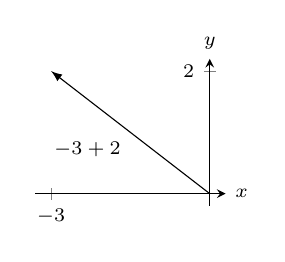
\begin{tikzpicture}[font=\scriptsize]
\begin{axis}[width=4cm,axis lines=middle,xlabel={$x$},ylabel={$y$},xlabel style={at={(current axis.right of origin)},anchor=west},ylabel style={at={(current axis.above origin)},anchor=south},xtick={-3},ytick={2},enlargelimits=true]
\addplot[-latex] plot coordinates {(0,0)(-3,2)}node[pos=0.5,below left]{$-3\ai+2\aj$};
\end{axis}
\end{tikzpicture}
\caption{}
\label{شکل_سوال_سمتیہ_نقطہ_الف}
\end{minipage}\hfill
\begin{minipage}{0.22\textwidth}
\centering
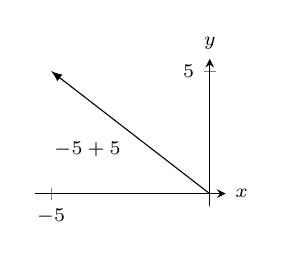
\begin{tikzpicture}[font=\scriptsize]
\begin{axis}[width=4cm,axis lines=middle,xlabel={$x$},ylabel={$y$},xlabel style={at={(current axis.right of origin)},anchor=west},ylabel style={at={(current axis.above origin)},anchor=south},xtick={-5},ytick={5},enlargelimits=true]
\addplot[-latex] plot coordinates {(0,0)(-5,5)}node[pos=0.5,below left]{$-5\ai+5\aj$};
\end{axis}
\end{tikzpicture}
\caption{}
\label{شکل_سوال_سمتیہ_نقطہ_ب}
\end{minipage}\hfill
\begin{minipage}{0.22\textwidth}
\centering
\begin{tikzpicture}[font=\scriptsize]
\begin{axis}[width=4cm,axis lines=middle,xlabel={$x$},ylabel={$y$},xlabel style={at={(current axis.right of origin)},anchor=west},ylabel style={at={(current axis.above origin)},anchor=south},xtick={1},ytick={-4},enlargelimits=true]
\addplot[-latex] plot coordinates {(0,0)(1,-4)}node[pos=0.5,below left]{$\ai-4\aj$};
\end{axis}
\end{tikzpicture}
\caption{}
\label{شکل_سوال_سمتیہ_نقطہ_پ}
\end{minipage}\hfill
\begin{minipage}{0.22\textwidth}
\centering
\begin{tikzpicture}[font=\scriptsize]
\begin{axis}[clip=false,width=4cm,axis lines=middle,xlabel={$x$},ylabel={$y$},xlabel style={at={(current axis.right of origin)},anchor=west},ylabel style={at={(current axis.above origin)},anchor=south},xtick={-1,1},ytick={-1,1},enlargelimits=true]
\addplot[-latex] plot coordinates {(0,0)(1,1)}node[above left]{$\krightharpoonup{AB}$};
\addplot[-latex] plot coordinates {(0,0)(-1,-1)}node[below right]{$\krightharpoonup{CD}$};
\addplot[]plot coordinates {(0,0)}node[circ]{}node[pin={[font=\tiny,pin distance=0.1cm]135:{$\krightharpoonup{AB}+\krightharpoonup{CD}=0$}}]{};
\end{axis}
\end{tikzpicture}
\caption{}
\label{شکل_سوال_سمتیہ_نقطہ_ت}
\end{minipage}
\end{figure}
\موٹا{اکائی سمتیات}\\
سوال \حوالہ{سوال_سمتیہ_اکائی_الف} تا سوال \حوالہ{سوال_سمتیہ_اکائی_پ} میں دیے سمتیات ترسیم کریں۔ ان سمتیات کو \عددی{a\ai+b\aj} روپ میں لکھیں۔

\ابتدا{سوال}\شناخت{سوال_سمتیہ_اکائی_الف}
زاویہ \عددی{\theta=\tfrac{\pi}{6}} اور \عددی{\theta=\tfrac{2\pi}{3}} کے لئے اکائی سمتیات \عددی{\kvec{u}=(\cos\theta)\ai+(\sin\theta)\aj} ترسیم کریں۔ دائرہ \عددی{x^2+y^2=1} کی ترسیم بھی شامل کریں۔\\
جواب:\quad
شکل \حوالہ{شکل_سوال_سمتیہ_اکائی_الف}
\انتہا{سوال}
%===================
\ابتدا{سوال}
زاویہ \عددی{\theta=-\tfrac{\pi}{4}} اور \عددی{\theta=-\tfrac{3\pi}{4}} کے لئے اکائی سمتیات \عددی{\kvec{u}=(\cos\theta)\ai+(\sin\theta)\aj} ترسیم کریں۔ دائرہ \عددی{x^2+y^2=1} کی ترسیم بھی شامل کریں۔
\انتہا{سوال}
%======================
\ابتدا{سوال}\شناخت{سوال_سمتیہ_اکائی_ب}
سمتیہ \عددی{\aj} کو مبدا کے گرد گھڑی کے الٹ رخ \عددی{\tfrac{3\pi}{4}} ریڈیئن  گھما کر حاصل اکائی سمتیہ ترسیم کریں۔\\
جواب:\quad
شکل \حوالہ{شکل_سوال_سمتیہ_اکائی_ب}
\انتہا{سوال}
%===================
\ابتدا{سوال}\شناخت{سوال_سمتیہ_اکائی_پ}
سمتیہ \عددی{\aj} کو مبدا کے گرد گھڑی کے رخ \عددی{\tfrac{2\pi}{3}} ریڈیئن  گھما کر حاصل اکائی سمتیہ ترسیم کریں۔
\انتہا{سوال}
%===================
\begin{figure}
\centering
\begin{minipage}{0.22\textwidth}
\centering
\begin{tikzpicture}[font=\tiny]
\begin{axis}[clip=false,axis equal,width=4cm,axis lines=middle,xlabel={$x$},ylabel={$y$},xlabel style={at={(current axis.right of origin)},anchor=west},ylabel style={at={(current axis.above origin)},anchor=south},xtick={1},ytick={\empty},enlargelimits=true]
\addplot[-latex,thick,data cs=polar]plot coordinates{(0,0)(30,1)}node[above,xshift=2ex,yshift=1ex]{$\kvec{u}=\tfrac{\sqrt{3}}{2}\ai+\tfrac{1}{2}\aj$};
\addplot[-latex,thick,data cs=polar]plot coordinates{(0,0)(120,1)}node[above,xshift=-3ex]{$\kvec{u}=-\tfrac{1}{2}\ai+\tfrac{\sqrt{3}}{2}\aj$};
\addplot[domain=0:360]({1*cos(x)},{1*sin(x)});
\addplot[-stealth,domain=0:30]({0.5*cos(x)},{0.5*sin(x)})node[pos=0.6,right]{$\tfrac{\pi}{6}$};
\addplot[-stealth,domain=0:120]({0.3*cos(x)},{0.3*sin(x)})node[pos=0.5,above]{$\tfrac{2\pi}{3}$};
\end{axis}
\end{tikzpicture}
\caption{}
\label{شکل_سوال_سمتیہ_اکائی_الف}
\end{minipage}\hfill
\begin{minipage}{0.22\textwidth}
\centering
\begin{tikzpicture}[font=\tiny]
\pgfmathsetmacro{\k}{-1/sqrt(2)}
\begin{axis}[clip=false,axis equal,width=4cm,axis lines=middle,xlabel={$x$},ylabel={$y$},xlabel style={at={(current axis.right of origin)},anchor=west},ylabel style={at={(current axis.above origin)},anchor=south},xtick={\k},ytick={\k},xticklabels={$-\tfrac{\sqrt{2}}{2}$},yticklabels={$-\tfrac{\sqrt{2}}{2}$},enlargelimits=true]
\addplot[-latex]plot coordinates {(0,0)(\k,\k)}node[pos=0.5,left]{$-\tfrac{\sqrt{2}}{2}\ai-\tfrac{\sqrt{2}}{2}\aj$};
\end{axis}
\end{tikzpicture}
\caption{}
\label{شکل_سوال_سمتیہ_اکائی_ب}
\end{minipage}\hfill
\begin{minipage}{0.22\textwidth}
\centering
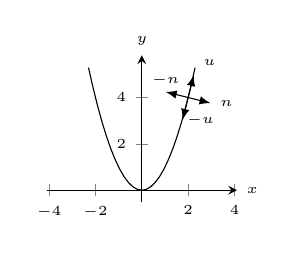
\begin{tikzpicture}[font=\tiny,declare function={f(\x)=(\x)^2;}]
\pgfmathsetmacro{\k}{1/sqrt(17)}
\begin{axis}[clip=false,axis equal,width=4cm,axis lines=middle,xlabel={$x$},ylabel={$y$},xlabel style={at={(current axis.right of origin)},anchor=west},ylabel style={at={(current axis.above origin)},anchor=south},enlargelimits=true]
\addplot[domain=-2.3:2.3]{f(x)};
\draw[-latex] (axis cs:2,4)--(axis cs:2+\k,4+4*\k)node[above right]{$\kvec{u}$};
\draw[-latex] (axis cs:2,4)--(axis cs:2-\k,4-4*\k)node[xshift=1.5ex]{$-\kvec{u}$};
\draw[-latex] (axis cs:2,4)--(axis cs:2+4*\k,4-\k)node[right]{$\kvec{n}$};
\draw[-latex] (axis cs:2,4)--(axis cs:2-4*\k,4+\k)node[yshift=1ex]{$-\kvec{n}$};
\end{axis}
\end{tikzpicture}
\caption{}
\label{شکل_سوال_سمتیہ_عمودی_مماسی_الف}
\end{minipage}\hfill
\begin{minipage}{0.22\textwidth}
\centering
\begin{tikzpicture}[font=\tiny,declare function={f(\x)=rad(atan(\x));}]
\pgfmathsetmacro{\k}{2/sqrt(5)}
\pgfmathsetmacro{\a}{pi/4}
\begin{axis}[clip=false,width=4cm,axis lines=middle,xlabel={$x$},ylabel={$y$},xlabel style={at={(current axis.right of origin)},anchor=west},ylabel style={at={(current axis.above origin)},anchor=south},enlargelimits=true, xtick={1},ytick={\a},yticklabels={$\tfrac{\pi}{4}$}]
\addplot[smooth,samples=100,domain=-1:2.5]{f(x)}node[below]{$y=\tan^{-1}(x)$};
\addplot[-latex] plot coordinates {(1,pi/4)(1+\k,pi/4+1/2*\k)}node[above]{$\kvec{u}$};
\addplot[-latex] plot coordinates {(1,pi/4)(1-\k,pi/4-1/2*\k)}node[left]{$-\kvec{u}$};
\addplot[-latex] plot coordinates {(1,pi/4)(1+1/2*\k,pi/4-\k)}node[below]{$\kvec{n}$};
\addplot[-latex] plot coordinates {(1,pi/4)(1-1/2*\k,pi/4+\k)}node[above]{$-\kvec{n}$};
\end{axis}
\end{tikzpicture}
\caption{}
\label{شکل_سوال_سمتیہ_عمودی_مماسی_ب}
\end{minipage}
\end{figure}
%==========================
سوال \حوالہ{سوال_سمتیہ_اکائی_گھوم_الف} اور سوال \حوالہ{سوال_سمتیہ_اکائی_گھوم_ب} میں اکائی سمتیہ \عددی{\kvec{u}=(\cos\theta)\ai+(\sin\theta)\aj} اسی رخ تلاش کریں۔

\ابتدا{سوال}\شناخت{سوال_سمتیہ_اکائی_گھوم_الف}
$6\ai-8\aj$\\
جواب:\quad
$\tfrac{3}{5}\ai-\tfrac{4}{5}\aj$
\انتہا{سوال}
%==================
\ابتدا{سوال}\شناخت{سوال_سمتیہ_اکائی_گھوم_ب}
$-\ai+3\aj$
\انتہا{سوال}
%=====================

سوال \حوالہ{سوال_سمتیہ_عمودی_مماسی_الف} تا سوال \حوالہ{سوال_سمتیہ_عمودی_مماسی_پ} میں دیے گئے نقطہ پر منحنی کے مماسی اکائی سمتیات اور عمودی اکائی سمتیات تلاش کریں۔ منحنی اور اکائی سمتیات کو ایک ساتھ ترسیم کریں۔ (سمتیات کی تعداد چار ہو گی۔)

\ابتدا{سوال}\شناخت{سوال_سمتیہ_عمودی_مماسی_الف}
$y=x^2,\quad (2,4)$\\
جواب:\quad
$\kvec{u}=\tfrac{1}{\sqrt{17}}\ai+\tfrac{4}{\sqrt{17}}\aj,\quad -\kvec{u}=-\tfrac{1}{\sqrt{17}}\ai-\tfrac{4}{\sqrt{17}}\aj,$\\
$ \kvec{n}=\tfrac{4}{\sqrt{17}}\ai-\tfrac{1}{\sqrt{17}}\aj,\quad -\kvec{n}=-\tfrac{4}{\sqrt{17}}\ai+\tfrac{1}{\sqrt{17}}\aj$\quad
شکل \حوالہ{شکل_سوال_سمتیہ_عمودی_مماسی_الف}
\انتہا{سوال}
%======================
\ابتدا{سوال}
$x^2+2y^2=6,\quad (2,1)$
\انتہا{سوال}
%======================
\ابتدا{سوال}\شناخت{سوال_سمتیہ_عمودی_مماسی_ب}
$y=\tan^{-1}x,\quad (1,\tfrac{\pi}{4})$\\
جواب:\quad
$\kvec{u}=\tfrac{1}{\sqrt{5}}(2\ai+\aj),\quad -\kvec{u}=\tfrac{1}{\sqrt{5}}(-2\ai-\aj),$\\
$\kvec{n}=\tfrac{1}{\sqrt{5}}(-\ai+2\aj),\quad -\kvec{n}=\tfrac{1}{\sqrt{5}}(\ai-2\aj),$\quad 
شکل \حوالہ{شکل_سوال_سمتیہ_عمودی_مماسی_ب}
\انتہا{سوال}
%======================
\ابتدا{سوال}\شناخت{سوال_سمتیہ_عمودی_مماسی_پ}
$y=\sum_{n=0}^{\infty}\frac{x^n}{n!},\quad (0,1)$
\انتہا{سوال}
%======================
سوال \حوالہ{سوال_سمتیہ_عمودی_مماسی_نقطہ_الف} تا سوال \حوالہ{سوال_سمتیہ_عمودی_مماسی_نقطہ_ب} میں دیے گئے نقطہ پر منحنی کے مماسی اور عمودی اکائی سمتیات تلاش کریں۔ 

\ابتدا{سوال}\شناخت{سوال_سمتیہ_عمودی_مماسی_نقطہ_الف}
$3x^2+8xy+2y^2-3=0,\quad (1,0)$\\
جواب:\quad
$\kvec{u}=\pm\tfrac{1}{5}(-4\ai+3\aj),\quad \kvec{v}=\pm\tfrac{1}{5}(3\ai+4\aj)$
\انتہا{سوال}
%=====================
\ابتدا{سوال}
$x^2-6xy+8y^2-2x-1=0,\quad (1,1)$
\انتہا{سوال}
%=====================
\ابتدا{سوال}
$y=\int_{0}^{x}\sqrt{3+t^4}\dif t,\quad (0,0)$\\
جواب:\quad
$\kvec{u}=\pm\tfrac{1}{2}(\ai+\sqrt{3}\aj),\quad \kvec{v}=\pm\tfrac{1}{2}(-\sqrt{3}\ai+\aj)$
\انتہا{سوال}
%=====================
\ابتدا{سوال}\شناخت{سوال_سمتیہ_عمودی_مماسی_نقطہ_ب}
$y=\int_{e}^{x}\ln (\ln t)\dif t,\quad (e,0)$
\انتہا{سوال}
%=====================

\موٹا{لمبائی اور رخ}\\
سوال \حوالہ{سوال_سمتیہ_لمبائی_رخ_الف} اور سوال \حوالہ{سوال_سمتیہ_لمبائی_رخ_ب} میں دیے سمتیہ کو لمبائی ضرب رخ کی صورت میں لکھیں۔

\ابتدا{سوال}\شناخت{سوال_سمتیہ_لمبائی_رخ_الف}
$5\ai+12\aj$\\
جواب:\quad
$13(\tfrac{5}{13}\ai+\tfrac{12}{13}\aj)$
\انتہا{سوال}
%====================
\ابتدا{سوال}\شناخت{سوال_سمتیہ_لمبائی_رخ_ب}
$2\ai-3\aj$
\انتہا{سوال}
%====================
\ابتدا{سوال}
سمتیہ \عددی{3\ai-4\aj} کے متوازی دو اکائی سمتیات دریافت کریں۔\\
جواب:\quad
$\tfrac{3}{5}\ai-\tfrac{4}{5}\aj,\quad -\tfrac{3}{5}\ai+\tfrac{4}{5}\aj$
\انتہا{سوال}
%=======================
\ابتدا{سوال}
سمتیہ \عددی{\kvec{A}=-\ai+2\aj} کے مخالف رخ ایسا سمتیہ تلاش کریں جس کی لمبائی \عددی{2} ہو۔ ایسے کتنے سمتیات ممکن ہیں؟
\انتہا{سوال}
%=========================
\ابتدا{سوال}
دکھائیں کہ \عددی{\kvec{A}=3\ai+6\j} اور \عددی{\kvec{B}=-\ai-2\aj} ایک دوسرے کے مخالف رخ ہیں۔ دونوں کا خاکہ بنائیں۔
\انتہا{سوال}
%=======================
\ابتدا{سوال}
دکھائیں کہ \عددی{\kvec{A}=3\ai+6\j} اور \عددی{\kvec{B}=\tfrac{1}{2}\ai+\aj} کے رخ ایک دوسرے جیسے ہیں۔
\انتہا{سوال}
%=======================

\موٹا{نظریہ اور مثالیں}\\
\ابتدا{سوال}
آپ ایک ریڑھی کو قوت \عددی{\kvec{F}} سے کھینچ رہے ہیں جس کی مقدار \عددی{\abs{\kvec{F}}=\SI{10}{\newton}} ہے۔زمین کے ساتھ قوت کا زاویہ \عددی{30^{\circ}} ہے۔ اس قوت کے \عددی{x} اور \عددی{y} اجزاء تلاش کریں۔\\
جواب:\quad
$5\sqrt{3}\ai,\quad 5\aj$
\انتہا{سوال}
%===================
\ابتدا{سوال}
پتنگ کی ڈوری آپ کو زمین کے ساتھ \عددی{45^{\circ}} زاویہ پر \عددی{\SI{5}{\newton}} قوت سے کھینچتی ہے۔ اس قوت کے افقی اور انتصابی اجزاء تلاش کریں۔
\انتہا{سوال}
%===============
\ابتدا{سوال}\شناخت{سوال_سمتیہ_سمتیات_دیگر}
سمتیہ \عددی{\kvec{A}=2\ai+\aj}، \عددی{\kvec{B}=\ai+\aj} اور \عددی{\kvec{C}=\ai-\aj} دیے گئے ہیں۔ ایسے غیر سمتیات \عددی{\alpha} اور \عددی{\beta} کہ \عددی{\kvec{A}=\alpha\kvec{B}+\beta\kvec{C}} ہو۔\\
جواب:\quad
$\alpha=\tfrac{3}{2},\quad \beta=\tfrac{1}{2}$
\انتہا{سوال}
%=================
\ابتدا{سوال}
سمتیات \عددی{\kvec{A}=\ai-2\aj}، \عددی{\kvec{B}=2\ai+3\aj} اور \عددی{\kvec{C}=\ai+\aj} دیے گئے ہیں۔ سمتیہ \عددی{\kvec{A}=\kvec{A}_1+\kvec{A}_2} لکھیں جہاں \عددی{\kvec{A}_1} سمتیہ \عددی{\kvec{B}} کے متوازی اور \عددی{\kvec{A}_2} سمتیہ \عددی{\kvec{C}} کے متوازی ہے۔ (سوال \حوالہ{سوال_سمتیہ_سمتیات_دیگر} دیکھیں۔)
\انتہا{سوال}
%====================
\ابتدا{سوال}
 ایک پرندہ اپنے گھونسلے سے اڑ کر، مشرق سے شمال کی طرف \عددی{60^{\circ}} پر  \عددی{5} کلومیٹر دور ایک درخت پر آرام کے لئے بیٹھتا ہے۔ اس کے بعد یہ جنوب مشرق رخ \عددی{10} کلومیٹر دور ایک کھنبے پر اڑ کر  بیٹھتا ہے۔ مستوی \عددی{xy} کے مبدا پر گھونسلا، مثبت \عددی{x} محور پر مشرق اور مثبت \عددی{y} محور پر شمال  رکھ (ا) درخت کا مقام تلاش کریں۔ (ب) کھنبے کا مقام تلاش کریں۔\\
جواب:\quad
(ا) \عددی{(5\cos 60^{\circ},5\sin 60^{\circ})=(\tfrac{5}{2},\tfrac{5\sqrt{3}}{2}}،\\
 (ب) \عددی{(5\cos 60^{}+10\cos 315^{},5\sin 60^{\circ}+10\sin 315^{\circ})=(\tfrac{5+\sqrt{2}}{2},\tfrac{5\sqrt{3}-10\sqrt{2}}{2})}
\انتہا{سوال}
%===================
\ابتدا{سوال}
 ایک پرندہ اپنے گھونسلے سے اڑ کر، شمال مشرق رخ \عددی{7} کلومیٹر دور ایک درخت پر آرام کرتا ہے۔ اس کے بعد یہ مغرب سے  \عددی{30^{\circ}} زاویہ جنوب کے رخ \عددی{8} کلومیٹر دور ایک کھنبے پر اڑ کر بیٹھتا ہے۔ مستوی \عددی{xy} کے مبدا پر گھونسلا، مثبت \عددی{x} محور پر مشرق اور مثبت \عددی{y} محور پر شمال  رکھ (ا) درخت کا مقام تلاش کریں۔ (ب) کھنبے کا مقام تلاش کریں۔
\انتہا{سوال}
%===================
\ابتدا{سوال}
مستوی میں \عددی{\kvec{v}} ایک سمتیہ ہے جو \عددی{y} محور کے متوازی نہیں ہے۔ سمتیہ \عددی{\kvec{v}} کی ڈھلوان اور سمتیہ \عددی{-\kvec{v}} کی ڈھلوان کا آپس میں کیا تعلق ہو گا؟ اپنے جواب کی وجہ پیش کریں۔\\
جواب:\quad
\عددی{-\kvec{v}=-a\ai-b\aj} کی ڈھلوان \عددی{\tfrac{(-b)}{(-a)}} ہے۔ یہی \عددی{\kvec{v}} کی بھی ڈھلوان ہے۔
\انتہا{سوال}
%==============

\حصہ{کارتیسی (مستطیل) محدد اور فضا میں سمتیات}
ہم اب سہ بعدی کارتیسی محدد بیان کرتے ہیں اور فضا میں اپنا راستہ تلاش کرنا سیکھتے ہیں۔ ہم فاصلہ کی تعریف جانیں گے،  فضا میں سمتیات کے ساتھ کام کرنا (مستوی کے قواعد اب بھی لاگو ہوں گے، پس اب ایک محدد بڑھ جائے گا)، اور نقطوں کے سلسلہ کا مساوات اور عدم مساوات کے ساتھ تعلق سیکھیں گے۔

\جزوحصہء{کارتیسی محدد} 
فضا میں نقطہ کی تلاش کے لئے تین آپس میں عمودی محددی محور استعمال کیے جاتے ہیں۔  شکل میں محور \عددی{Ox}، \عددی{Oy} اور \عددی{Oz} دایاں ہاتھ محددی نظام دیتے ہیں۔ دائیں ہاتھ کے نظام میں، انگوٹھے کو باقی انگلیوں کے ساتھ زاویہ قائمہ پر رکھتے ہوئے، اگر آپ اپنے دائیں ہاتھ کی چار انگلیوں کو مثبت \عددی{x} محور پر رکھ کر انہیں مثبت \عددی{y} محور کی جانب موڑیں تب آپ کا انگوٹھا مثبت \عددی{z} محور پر ہو گا۔

فضا میں نقطہ \عددی{N} سے گزرتی، محوروں کے قائمہ سطحیں ان محور کو اعداد  \عددی{(x,y,z)} پر قطع کریں گی۔ یہی اعداد نقطہ \عددی{N} کے کارتیسی محدد ہوں گے۔  

محور \عددی{x} پر نقطوں کے \عددی{y} اور \عددی{z} محدد صفر ہوں گے لہٰذا ان کے محدد کی صورت \عددی{(x,0,0)} ہو گی۔ اسی طرح محور \عددی{y} پر نقطوں کے \عددی{x} اور \عددی{z} محدد صفر ہوں گے لہٰذا ان نقطوں کے محدد کی صورت \عددی{(0,y,0)} ہو گی۔ محور \عددی{z} پر نقطوں کے \عددی{x} اور \عددی{y} محدد صفر ہوں گے لہٰذا ان کے محددی کی صورت \عددی{(0,0,z)} ہو گی۔

محور \عددی{x} کے عمودی سطح پر تمام نقطوں کا \عددی{x} محدد وہی ہو گا جس \عددی{x} محدد  پر یہ سطح \عددی{x} محور کو قطع کرتا ہے۔ اس سطح پر نقطوں کے \عددی{y} اور \عددی{z} محدد کچھ بھی ہو سکتے ہیں۔ اسی طرح محور \عددی{y} کے عمودی سطح پر تمام نقطوں کا مشترک \عددی{y} محدد ہو گا اور  محور \عددی{z} کے عمودی سطح پر تمام نقطوں کا مشترک \عددی{z} محدد ہو گا۔ ان سطحوں کی مساوات لکھتے ہوئے ہم اس مشترکہ محدد کی قیمت لکھتے ہیں۔ یوں مستوی \عددی{x=2} محور \عددی{x} کو عمودی ہے اور یہ مستوی محور \عددی{x} کو نقطہ \عددی{x=2} پر قطع کرتا ہے۔ مستوی \عددی{y=3} محور \عددی{y} کو عمودی ہے اور اس کو نقطہ \عددی{y=3} پر قطع کرتا ہے۔مستوی \عددی{z=5} محور \عددی{z} کو عمودی ہے اور اس محور کو نقطہ \عددی{z=5} پر قطع کرتا ہے۔ شکل میں مستوی \عددی{x=2}، \عددی{y=3} اور \عددی{z=5} دکھائے گئے ہیں۔ ان کا مشترک نقطہ بھی دکھایا گیا ہے جہاں یہ تینوں ایک دوسرے کو قطع کرتے ہیں۔

مستوی \عددی{x=2} اور \عددی{y=3} ایک دوسرے کو ایک لکیر پر قطع کرتے ہیں جو محور \عددی{z} کے متوازی ہے۔ اس لکیر کو جوڑی مساوات \عددی{x=2}، \عددی{y=3} ظاہر کرتے ہیں۔ نقطہ \عددی{(x,y,z)} صرف اور صرف اس صورت اس لکیر پر پایا جائے گا جب \عددی{x=2} اور \عددی{y=3} ہوں۔ اسی طرح مستوی \عددی{y=3} اور \عددی{z=5} ایک لکیر پر ایک دوسرے کو قطع کرتے ہیں اور اس لکیر کو جوڑی مساوات \عددی{y=3}، \عددی{z=5} ظاہر کرتے ہیں۔ یہ لکیر محور \عددی{x} کے متوازی ہو گی۔ مستوی \عددی{x=2} اور \عددی{z=5} ایک لکیر پر ایک دوسرے کو قطع کرتے ہیں اور اس لکیر کو جوڑی مساوات \عددی{x=2}، \عددی{z=5} ظاہر کرتے ہیں۔ یہ لکیر محور \عددی{y} کے متوازی ہو گی۔

محددی محوروں کے بیچ \اصطلاح{مستوی \عددی{xy}}\فرہنگ{مستوی!ایکس وائے}\حاشیہب{xy-plane}\فرہنگ{plane!xy} جس کی معیاری مساوات \عددی{z=0}؛ \اصطلاح{مستوی \عددی{yz}} جس کی معیاری مساوات \عددی{x=0}؛ اور \اصطلاح{مستوی \عددی{xz}} جس کی معیاری مساوات \عددی{y=0} ہے پائی جاتی ہیں۔ یہ تینوں مستوی مبدا \عددی{(0,0,0)} پر آپس میں ملتے ہیں۔

تین \اصطلاح{محددی مستوی}\فرہنگ{مستوی!محددی}\حاشیہب{coordinate planes}\فرہنگ{planes!coordinate} \عددی{x=0}، \عددی{y=0} اور \عددی{z=0} فضا کو آٹھ حصوں میں تقسیم کرتے ہیں جنہیں \اصطلاح{ثُمن}\فرہنگ{ثمن}\حاشیہب{octant}\فرہنگ{octant} کہتے ہیں۔ وہ ثمن جس میں تمام محدد مثبت ہیں \اصطلاح{پہلا ثمن}\فرہنگ{ثمن!پہلا}\حاشیہب{first octant}\فرہنگ{octant!first} کہلاتا ہے۔ باقی سات ثمن کو نام دینے کا کوئی روایتی طریقہ نہیں پایا جاتا ہے۔

چونکہ فضا کے کارتیسی محدد ایک دوسرے کو زاویہ قائمہ پر ملتے ہیں لہٰذا ان محدد  کو \اصطلاح{مستطیل محدد}\فرہنگ{محدد!مستطیل}\حاشیہب{rectangular coordinates}\فرہنگ{coordinates!rectangular} بھی کہتے ہیں۔  

درج ذیل مثال میں ہم مساواتوں اور عدم مساواتوں کا خلا میں ہم پلہ نقطے تلاش کرتے ہیں۔ 
